\documentclass[a4paper,french,bookmarks]{book}

\usepackage{booktabs}
\usepackage{minitoc}
\usepackage{./Structure/4PE18TEXTB}
\usepackage{proof}
\usepackage{pdfpages}
\usepackage[version=4]{mhchem}

\makeatletter
\renewcommand*\l@section{\@dottedtocline{1}{1.8em}{3.5em}}
\renewcommand*\l@subsection{\@dottedtocline{2}{5.3em}{3.5em}}
\makeatother

\newboxans
\renewcommand{\thechapter}{\Roman{chapter}}
\renewcommand{\thesubsection}{\thesection.\Alph{subsection}}
\mtcsettitle{minitoc}{}

\DeclareDocumentCommand\NO{g}{\funlv{N.O.}{#1}}


\newcommand{\chaptertoc}[0]{
    \setcounter{tocdepth}{2}
    \begin{tcolorbox}[
        enhanced,
        frame hidden,
        sharp corners,
        detach title,
        spread outwards     = 5pt,
        halign              = center,
        valign              = center,
        borderline west     = {3pt}{0pt}{main20!50!main2!95!gray!90},
        coltitle            = main20!50!main2!95!gray!90, 
        interior style      = {
            left color      = main1white2!65!gray!11,
            middle color    = main1white2!50!gray!10,
            right color     = main1white2!35!gray!9
        },
        arc                 = 0 cm,
        title               = SOMMAIRE,
        boxrule             = 0pt,
        fonttitle           = \bfseries\sffamily,
        overlay             = {
            \node[rotate=90, minimum width=1cm, anchor=south,yshift=-0.8cm]
            at (frame.west) {\tcbtitle};
        }
    ]
        \begin{minipage}{0.83\linewidth}
            \sffamily
            \minitoc
        \end{minipage}
    \end{tcolorbox}
}

\begin{document}
    
    %==============================
    % METADONNEES
    %==============================
    
    \title{Cours de Physique de MPI/MPI* (2022-2023)}
    \author{SIAHAAN--GENSOLLEN Rémy}
    \date{\today}
    \hypersetup{
        pdftitle={Cours de Physique de MPI/MPI* (2022-2023)},
        pdfauthor={SIAHAAN--GENSOLLEN Rémy},
        pdflang={fr-FR},
        pdfsubject={MPI/MPI*, Cours de Physique},
        pdfkeywords={MPI/MPI*, Cours de Physique, 2022-2023}
        pdfstartview=
    }
    
    %==============================
    % MISE EN PAGE
    %==============================
    
    \titleformat{\chapter}[display]{\normalfont\huge\bfseries}{}{0pt}{
        \begin{tcolorbox}[
            enhanced,
            frame hidden,
            sharp corners,
            spread sidewards    = 5pt,
            halign              = center,
            valign              = center,
            interior style      = {color=main1!20},
            arc                 = 0 cm,
            fontupper           = \color{black}\sffamily\bfseries\huge,
            fonttitle           = \normalfont\color{white}\sffamily\small,
            top                 = 1cm, 
            bottom              = 0.7cm,
            title               = Chapitre \thechapter,
            attach boxed title to bottom center = {
                yshift=\tcboxedtitleheight/2,
            },
            boxed title style = {
                frame code={
                \path[left color=main2!95!gray!90,
                right color=main1!95!gray!90] 
                    ([xshift=-10mm]frame.north west) -- 
                    ([xshift=10mm]frame.north east) -- 
                    ([xshift=10mm]frame.south east) -- 
                    ([xshift=-10mm]frame.south west) -- 
                    cycle;
                },
                interior engine=empty
            }
        ]
            #1
        \end{tcolorbox}%
    }
    \titlespacing*{\chapter}{0pt}{-120pt}{-15pt}
    \titleformat{name=\chapter,numberless}[display]{\normalfont\huge\bfseries}
    {}{0pt}{
        \begin{tcolorbox}[
            enhanced,
            frame hidden,
            sharp corners,
            spread sidewards    = 5pt,
            halign              = center,
            valign              = center,
            interior style      = {color=main1!20},
            arc                 = 0 cm,
            outer arc           = 0pt,
            leftrule            = 0pt,
            rightrule           = 0pt,
            fontupper           = \color{black}\sffamily\bfseries\huge,
            enlarge left by     = -1in-\hoffset-\oddsidemargin, 
            enlarge right by    = -\paperwidth+1in+\hoffset +
            \oddsidemargin+\textwidth,
            width               = \paperwidth, 
            left                = 1in+\hoffset+\oddsidemargin, 
            right               = \paperwidth-1in-\hoffset -
            \oddsidemargin-\textwidth,
            top                 = 1cm, 
            bottom              = 1cm
        ]
            #1
        \end{tcolorbox}%
    }
    \titlespacing*{name=\chapter,numberless}{0pt}{-115pt}{0pt}
    
    %==============================
    % PREMIERE DE COUVERTURE
    %==============================

    \includepdf[pages={1},scale=1.15,offset=0mm -18mm]{CPCover.pdf}
    
    %==============================
    % PAGE VIDE
    %==============================
    
    \pagestyle{empty}
    
    %==============================
    % PAGE DE COUVERTURE INTERNE
    %==============================
    
    \begin{titlepage}
	    \begin{center}
	        {\scshape SIAHAAN--GENSOLLEN Rémy\par}
	        \vspace{2cm}
	        {\huge\sffamily Cours de\par}
	        \vspace{0.5cm}
	        {\Huge\bfseries\sffamily PHYSIQUE\par}
	        \vspace{1cm}
	        {\Large\textit{donné pendant mon année de \textsf{MPI/MPI*} à
	        Janson-de-Sailly}\\[5pt]\texttt{(2022-2023)}\par}
	        \vfill
	        {\large\EBGaramond Dernière compilation le \today\par}
        \end{center}
    \end{titlepage}
    
    %==============================
    % PAGE VIDE
    %==============================
    
    \pagestyle{empty}\text{}\newpage
    
    %==============================
    % STYLE DES EN-TÊTES ET PIEDS DE PAGES
    %==============================
    
    \renewcommand\chaptermark[1]{\markboth{#1}{}}
    
    \fancypagestyle{intro}{
        \fancyhf{}
        \renewcommand{\headrulewidth}{0pt}
        \renewcommand{\footrulewidth}{0pt}\fancyfoot[RO,LE]{\GillSansMTMedium\color{white5}\thepage\;/\;\pageref{LastPage}}
        \fancyhead[LE]{\GillSansMTMedium\color{white5}\bfseries COURS DE PHYSIQUE}
        \fancyhead[RE]{\GillSansMTMedium\color{white5}Avant-propos}
        \fancyhead[LO]{\GillSansMTMedium\color{white5}\rightmark}
        \fancyhead[RO]{\GillSansMTMedium\color{white5}\textbf{MPI/MPI*} 2022-2023 \quad Janson-de-Sailly}
    }
    
    \fancypagestyle{toc}{
        \fancyhf{}
        \renewcommand{\headrulewidth}{0pt}
        \renewcommand{\footrulewidth}{0pt}\fancyfoot[RO,LE]{\GillSansMTMedium\color{white5}\thepage\;/\;\pageref{LastPage}}
        \fancyhead[LE]{\GillSansMTMedium\color{white5}\bfseries COURS DE PHYSIQUE}
        \fancyhead[RE]{\GillSansMTMedium\color{white5}Table des matières}
        \fancyhead[LO]{\GillSansMTMedium\color{white5}\rightmark}
        \fancyhead[RO]{\GillSansMTMedium\color{white5}\textbf{MPI/MPI*} 2022-2023 \quad Janson-de-Sailly}
    }
    
    \fancypagestyle{plain}{
        \fancyhf{}
        \renewcommand{\headrulewidth}{0pt}
        \renewcommand{\footrulewidth}{0pt}\fancyfoot[RO,LE]{\GillSansMTMedium\color{white5}\thepage\;/\;\pageref{LastPage}}
        \fancyhead[LE]{\GillSansMTMedium\color{white5}\bfseries COURS DE PHYSIQUE}
        \fancyhead[RE]{\GillSansMTMedium\color{white5}Chapitre \thechapter : \nouppercase{\leftmark}}
        \fancyhead[LO]{\GillSansMTMedium\color{white5}\nouppercase{\rightmark}}
        \fancyhead[RO]{\GillSansMTMedium\color{white5}\textbf{MPI/MPI*} 2022-2023 \quad Janson-de-Sailly}
    }
    
    %==============================
    % PREFACE 
    %==============================
    
    \chapter*{Avant-propos}
    \thispagestyle{intro}
    \addcontentsline{toc}{chapter}{Avant-propos}
    
    \text{\Large\EBGaramond\itshape À tout lecteur potentiel, quelques mots...}\newline\newline\newline
    
    \begin{center}
        \begin{minipage}{0.85\linewidth}
            \large \qquad Comme son nom l'indique, l'objectif de cet ouvrage est de fournir un cours de physique ~NEGRE~ en accord avec le programme des classes préparatoires \textsf{MPI/MPI*}. Il contiendra principalement des notes de cours, dont je serai dispensé mon année de \guill{spé'} (année 2022/2023) à \textit{Janson-de-Sailly}, par M. \textsc{Marc Antoine Blain}. J'essaierai par ailleurs de détailler et d'enrichir le plus possible son contenu au fil de l'année, à l'aide de mes cours de première année, d'autres ouvrages et de recherches en général. La rédaction de ce cours constitue un important projet, d'autant plus que j'en mène un similaire pour les enseignements de mathématiques et de physique cette année. C'est un travail qui peut s'avérer extrêmement chronophage, aussi risque-t-il d'être rarement mené jusqu'au bout.\newline
    
            \qquad Je ne prétends à aucun moment être enseignant, et ce livre reste avant tout destiné à mon usage personnel, aussi j'aviserai tout lecteur potentiel à faire preuve de prudence lors du parcours de ce texte, à ne pas hésiter à en vérifier le contenu par lui même. Il est très probable que de multiples erreurs (en tout genre) se soient glissés durant la rédaction, que je n'aurait su repérer, ou que le manque de temps empêche la correction. N'hésitez d'ailleurs pas à me le signaler, ou à me faire part de vos remarques en général.\newline
    
            \qquad J'espère enfin, et malgré les points exprimés précédemment, que ce cours pourra avoir une quelconque utilité à ceux qui s'y aventureraient, que sa lecture et son style en seront agréable (la mise en page et la composition graphique en général sont de ma conception personnelle, enrichie par les retours de mes camarades, et le fruit de plusieurs mois d'apprentissage de \LaTeX) et enrichissante.\newline\newline\newline\text{}
        \end{minipage}
    \end{center}
    
    \hfill{\large\textsc{Siahaan--Gensollen Rémy}}
    
    \pagestyle{intro}
    
    %==============================
    % TABLE DES MATIERES
    %==============================
    
    \newpage
    \dominitoc\nomtcrule 
    {\sffamily\tableofcontents}\mtcaddchapter\pagestyle{toc}
    
    \cleardoublepage
    
    %==============================
    % COURS
    %==============================
    
    \pagestyle{plain}
    
    \chapter{Quelques notions indispensables}
    
    Ce premier chapitre n'en est pas vraiment un. Il concerne surtout l'introduction et le rappel de plusieurs notions mathématiques (fonctions à plusieurs variables, équations différentielles, mesures, ...) qui seront important à l'enseignement de physique cette année. Il introduira également des opérateurs qui seront nécessaire dans des chapitres plus éloignés (gradient, rotationnel, ...)
    
    \chaptertoc
    
    \section{Fonctions à plusieurs variables}
    
    \subsection{Définition}
    
    On a déjà une bonne compréhension des fonctions à une variable. On prend généralement une fonction de la variable réelle, à valeur dans les réels, selon : 
    
    \[ f : \begin{array}[t]{rcl}
        \bdR &\to& \bdR  \\
        x &\mapsto& f\p{x} 
        \end{array}
    \]
    
    Pour construire une fonction à plusieurs variable, plutôt que de prendre une fonction de la variable réelle, on peut par exemple prendre une fonction d'un couple à valeur dans les réels :
    
    \[ f : \begin{array}[t]{rcl}
        \bdR^2 &\to& \bdR  \\
        \p{x, y} &\mapsto& f\p{x,y} 
        \end{array}
    \]
    
    Plus généralement, on peut définir :
    
    \begin{definition}{Fonction à plusieurs variables}
        Soit \hg{un entier $n \in \bdN$}, avec $n \geq 2$. On appelle \hg{fonctions à plusieurs variables} une fonction \hg{$f \in \bcF\p{\bdR^n, \bdR}$}, soit :
        
        \[ \hg{f : \begin{array}[t]{rcl}
        \bdR^n &\to& \bdR  \\
        \p{x_1, x_2, \dots, x_n} &\mapsto& f\p{x_1, x_2, \dots, x_n} 
        \end{array}}\]
    
    \end{definition}
    
    Généralement, les fonctions en physique seront fonctions de grandeurs physiques (masse, longueur, ...). Il n'y a qu'en physique quantique que l'on aura des fonctions complexes, principalement la fonction d'onde livrée par l'équation de \textsc{Schrödinger} :
    
    \[ \displaystyle \ii\hbar {\frac {\partial \Psi (t,{\vec {r}})}{\partial t}}=-{\frac {\hbar ^{2}}{2m}}\Delta \Psi (t,{\vec {r}})+V({\vec {r}})\Psi (t,{\vec {r}}) \]
    
    Il est très facile d'avoir des fonctions à plusieurs variables en physique. 
    
    \begin{example}{}{}
        Soit une résistante $R$, et \hg{$\bsE_J$ l'énergie dégagée par effet joule}. $\bsE_J$ a pour expression :
        %
        \[ \hg{\bsE_J = RI^2t} \]
        %
        Ainsi $\bsE_J$ est une \hg{fonction à trois variables} :
        %
        \[ \hg{\bsE_J = f\p{R, I, T}} \]
        %
        On peut également prendre \hg{$R$ comme un paramètre}, et l'on aurait alors :
        %
        \[ \hg{\bsE_J = g_R\p{I, T}} \]
        %
        Ainsi on aurait une \hg{fonction à deux variables}.
    \end{example}
    
    \subsection{Dérivées partielles}
    
    Pour rappel, si l'on a une fonction $y = f\p{x}$ à une seule variable $x$, on peut noter sa dérivée par rapport à $x$ :
    
    \begin{notation}
        $\dfrac{\dif y}{\dif x} = f'\p{x}$
    \end{notation}
    
    Lorsque c'est une fonction du temps $t$, on peut également la noter avec un point :
    
    \begin{notation}
        $\dot f\p{t} = \dfrac{\dif f}{\dif t}$
    \end{notation}
    
    Pour les fonctions à plusieurs variables, on peut également introduire une notion de dérivation.
    
    \begin{definition}{Dérivée partielle}
        La dérivée partielle de $f\p{x, y}$ par rapport à $x$ est la dérivée de $f$ par rapport à $x$ en maintenant $y$ constant.
    \end{definition}
    
    \begin{notation}
        La dérivée partielle de $f\p{x, y}$ par rapport à $x$ se note $\p{\dfrac{\partial f}{\partial x}}_y$ ou $\left.\dfrac{\partial f}{\partial x}\right\vert_y$.
    \end{notation}
    
    \begin{theorem}{Théorème de Schwarz}{}
        Si $f\p{x, y}$ est telle que $\dfrac{\partial^2 f}{\partial x^2}$ et $\dfrac{\partial^2 f}{\partial y^2}$ sont continues, alors on a :
        %
        \[ \p{\dfrac{\partial}{\partial y}\p{\p{\dfrac{\partial f}{\partial x}}_y}}_x = \p{\dfrac{\partial}{\partial x}\p{\p{\dfrac{\partial f}{\partial y}}_x}}_y \]
    \end{theorem}
    
    \textit{en gros}, le théorème de \textsc{Schwarz} dit que :
    %
    \[ \dfrac{\partial^2 f}{\partial y \partial x} = \dfrac{\partial^2 f}{\partial x \partial y}\]
    
    \subsection{Fonctions composées}
    
    Pour rappel, si l'on a trois fonctions $g$, $u$ et $v$ tel que $g = u \circ v$, \ie $g\p{x} = u\p{v\p{x}}$, alors on peut dériver selon :
    %
    \[ g'\p{x} = v'\p{x} \times u'\p{v\p{x}}\]
    
    On peut alors généraliser ce résultat. Si $\varphi\p{x, y} = f\p{u\p{x, y}, v\p{x, y}, w\p{x, y}}$, alors :
    %
    \[ \dep{\dfrac{\partial \varphi}{\partial x}}_y = \dep{\dfrac{\partial f}{\partial u}}_{v, w}\dep{\dfrac{\partial u}{\partial x}}_y + \dep{\dfrac{\partial f}{\partial v}}_{u, w}\dep{\dfrac{\partial v}{\partial x}}_y + \dep{\dfrac{\partial f}{\partial w}}_{u, v}\dep{\dfrac{\partial w}{\partial x}}_y\]
    
    \subsection{Différentielle totale}
    
    Cette partie est particulièrement importante.
    
    \begin{definition}{}{}
        Soit $f\p{x, y, z}$. Sa différentielle totale s'écrit :
        %
        \[ \dif f = \dep{\dfrac{\partial f}{\partial x}}_{y, z} \dif x + \dep{\dfrac{\partial f}{\partial y}}_{x, z} \dif y + \dep{\dfrac{\partial f}{\partial z}}_{x, y} \dif z \]
    \end{definition}
    
    L'intérêt d'une telle définition est de pouvoir calculer :
    %
    \[ \int_A^B \dif f = f\p{B} - f\p{A}\]
    %
    Qui est indépendant du chemin de $A$ à $B$.
    
    \begin{theorem}{}{}
        Soit $\delta \varphi\p{x, y, z} = P\p{x, y, z}\dif x + Q\p{x, y, z}\dif y + R\p{x, y, z}\dif z$.
        
        \[ \exists f,\qquad \delta \varphi = \dif f \iff \dfrac{\partial P}{\partial y} = \dfrac{\partial Q}{\partial x} \et \dfrac{\partial P}{\partial z} = \dfrac{\partial R}{\partial x} \et \dfrac{\partial Q}{\partial z} = \dfrac{\partial R}{\partial y}\]
        
        Soit $\implies P = \dfrac{\partial f}{\partial x} \qquad Q = \dfrac{\partial f}{\partial y} \qquad \partial \dfrac{\partial f}{\partial z}$
    \end{theorem}
    
    Application/exemple : savoir si une force est conservative :
    %
    \[ \delta W_{\vec{F}} = \vec{F} \cdot \dif \vec{M} = F_x\p{x, y, z}\dif x + F_y\p{x, y, z}\dif y + F_z\p{x, y, z}\dif z\]
    %
    Si $\dfrac{\partial F_x}{\partial y} = \dfrac{\partial F_y}{\partial x}$ et $\dfrac{\partial F_x}{\partial z} = \dfrac{\partial F_z}{\partial x}$ et $\dfrac{\partial F_y}{\partial z} = \dfrac{\partial F_z}{\partial x}$ alors :
    %
    \[ \exists E_p\p{x, y, z} \ \text{tel que}\qquad \delta W_{\vec{F}} = -\dif E_p\]
    %
    Avec $F_x = -\dfrac{\partial E_p}{\partial x}$, $F_y = -\dfrac{\partial E_p}{\partial y}$, $F_z = -\dfrac{\partial E_p}{\partial z}$ et $\vec{F} = -\vec{\nabla} E_p = -\vec{\grad} E_p$.
    
    \begin{warning}{}{}
        Intégrer une fonction à plusieurs variables (comme on pourrait le faire pour l'énergie potentielle) n'est pas évident, et bien moins simple que pour une fonction ) une seule variable.
    \end{warning}
    
    Une première méthode : 
    %
    \[ \dfrac{\partial f}{\partial x} = P\p{x, y} \implies f\p{x, y} = \int P\p{x, y} \dif x + g\p{y} \]
    
    et donc :
    
    \[ \dfrac{\partial f}{\partial y} = Q\p{x, y} = \dfrac{\partial}{\partial y } \int P\p{x, y} \dif x + \dfrac{\dif g\p{y}}{\dif y}\]
    
    Ainsi :
    %
    \[ \dfrac{\dif g\p{y}}{\dif y} = -\p{\dfrac{\partial}{\partial y}\int P\p{x, y}\dif x} + Q\p{x, y}\]
    
    Comme $F\p{x, y} = F\p{y}$, on a $g\p{y} = \int F\p{y}\dif y$.
    
    Une deuxième méthode consiste à construire un chemin de $M_0\p{x_0, y_0}$ à $M\p{x, y}$ :
    %
    \[ \dif f = f\p{x, y}\dif x + Q\p{x, y}\dif y\]
    
    Alors $\displaystyle f\p{x, y} - f\p{x_0, y_0} = \int_{x_0}^x \dif f\p{x, y_0} + \int_{y_0}^y \dif f \p{x, y}$.
    
    \section{Mesures physiques}
    
    \subsection{Généralité}
    
    Soit $X$ une grandeur physique, sa mesure s'obtient en la comparant à une grandeur de même nature choisit comme unité. $x$ est le résultat de la mesure de $X$, et l'on écrit $X = x$. Par exemple, $\ell = \SI{3.0}{\m} \implies \ell \in \intc{2,95 ; 3.05} \ \text{m}$. Ou encore $\ell = \SI{3.333333333}{\m}$.
    
    \subsection{Équations aux dimesions}
    
    Rappel sur les unité fondamentales (SI) :
    %
    \begin{enumerate}
        \begin{minipage}{0.45\linewidth}
            \itt Masse
            \itt Longeur
            \itt Temps
            \itt Intensité électrique
            \itt Quantité de matière
            \itt Température
        \end{minipage}
        %
        \hfill
        %
        \begin{minipage}{0.45\linewidth}
            \itt kilogramme
            \itt mètre
            \itt seconde
            \itt Ampère
            \itt mol
            \itt Kelvin
        \end{minipage}
    \end{enumerate}
    
    Soit une loi physique qui relie une grandeur physique $G$ à des grandeurs physiques $A$, $B$, $C$, \dots, sous la forme :
    %
    \[ G = k A^\alpha B^\beta, C^\gamma \dots\]
    %
    Avec $k$ un facteur numérique constant. $G$ a la même dimension que les dimensions de $A$, $B$, $C$, \dots élevées aux puissances $\alpha$, $\beta$, $\gamma$, \dots. ON note :
    %
    \[ \intc{G} \equiv \intc{A}^\alpha \intc{B}^\beta \intc{C}^\gamma \dots\]
    
    Ceci a trois intérêts :
    %
    \begin{enumerate}
        \item Changement d'unité. Par exemple, le \textit{dyre} est l'unité de force dans le système \textsc{CGS} (centimètre gramme seconde). On veut exprimer un dyre en Newtons. On a l'équation aux dimensions suivante :
        %
        \[ \intc{F} \equiv \textsf{M} \cdot \textsf{L} \cdot \textsf{T}^{-2}\]
        %
        Donc $\dfrac{\SI{1}{N}}{1 \ \text{dyre}} = \dfrac{\SI{1}{\kg} \cdot \SI{1}{\m\cdot\second^{-2}}}{\SI{1}{\g}\cdot \SI{1}{\cm \cdot \second^{-2}}} = \dfrac{10^3}{1} \times \dfrac{1}{10^{-2} = 10^5}$. Ainsi $\SI{1}{N} = \SI{1e5}{dyre}$ et $\SI{1}{dyre} = \SI{1e5}{N}$.
        
        \item Vérification de l'homogénéité des formules. Considérons la formule :
        
        \[ T = 2\pi \sqrt{\dfrac{\ell}{g}}\]
        
        On a l'équation aux dimensions :
        %
        \[ \intc{T} \equiv \dfrac{\intc{\ell}^{\sfrac{1}{2}}}{\intc{g}^{\sfrac{1}{2}}} \implies \textsf{T} \equiv \dfrac{\textsf{L}^{\sfrac{1}{2}}}{\textsf{L}^{\sfrac{1}{2}}\cdot \p{\textsf{T}^{-2}}^{\sfrac{1}{2}}} \equiv \textsf{T}\]
        
        L'équation est bien valide.
        
        \item Fréquence $\nu$ d'une corde de guitare. On a $\nu = f\p{L, F, \mu}$ avec $L$ la longueur de la corde, $F$ sa tension et $\mu$ sa masse linéique. On a alors :
        %
        \[ \nu = kL^\alpha F^\beta \mu^\gamma\]
        %
        L'équation aux dimensions donne :
        %
        \[ \textsf{T}^{-1} \equiv \textsf{L}^{\alpha} \cdot \p{\textsf{M} \cdot \textsf{L} \cdot \textsf{L}^{-2}}^\beta \cdot \p{\textsf{M} \cdot \textsf{L}^{-1}}^\gamma\]
        %
        On obtient alors le système :
        %
        \[ \left\lbrace\begin{array}{rcl}
            -1 &=& -2b  \\
            0 &=& a + b + c\\
            0 &=& b + c
        \end{array}\right. \iff \left\lbrace\begin{array}{rcl}
            b &=& \sfrac{1}{2}  \\
            c &=& -\frac{1}{2}\\
            a &=& -1
        \end{array}\right. \]
        %
        Ce qui amène enfin $\nu = k\dfrac{1}{L}\sqrt{\dfrac{F}{\mu}}$.
        
        (Schéma) On cherche $\theta_\text{décollage} = \theta_d$.
        
        \[ \theta_d = f\p{R, m, g} = kR^\alpha m^\beta g^\gamma\]
        
        \[ \textsf{\theta} \equiv \textsf{L}^\alpha \cdot \textsf{M}^\beta \cdot \p{\textsf{L} \cdot \textsf{T}^{-2}}^\gamma\]
        
        \[ \left\lbrace\begin{array}{rcl}
            0 &= a + c  \\
            0 &=& b \\
            0 &=& -2c
        \end{array}\right. \implies a = b = c = 0\]
    \end{enumerate}
    
    \subsection{Incertitudes}
    
    \subsubsection{Définition}
    
    Dans les dernières versions des programmes, les notions d'incertitude ont tendance à être \guill{à la mode}. Rappelons que l'important reste avant tout de ne pas donner de valeur numérique qui semble ridicule au yeux du correcteur. Mais l'on introduit également dans cette sous-section quelques notions plus précises (sans faire une introduction à la métrologie) concernant les incertitudes.
    
    \begin{definition}{Incertitude}{}
        Soit une grandeur $X$, de mesure $x$. $u\p{x}$ est l'écart type lié à la variabilité de la mesure.
        
        $u\p{x}$ évalue l'ordre de grandeur de l'incertitude de la mesure de $X$.
    \end{definition}
    
    Pour évaluer les incertitudes, il existe deux \guill{types} :
    
    \begin{enumerate}
        \itt Type A : on fait $N$ mesures. $x = \phyavg{x_i}$ et $u\p{x} = \sqrt{\phyavg{{x_i}^2}}$
        
        \itt Type B : propagation d'incertitude. Avec $X = f\p{X_1, X_2, \dots}$ et $u\p{x} = g\p{u\p{x_i}}$. On a :
        
        \[ X = \dfrac{X_1}{X_2} \lor X = X_1X_2\implies \dfrac{u\p{x}}{x} = \sqrt{\p{\dfrac{u\p{x_1}}{x_1}}^2 + \p{\dfrac{u\p{x_2}}{x_2}}^2}\]
        
        \[ X = X_1 + X_2 \implies u\p{x} = u\p{x_1} + u\p{x_2}\]
        
        \[ X = Y^n \implies \dfrac{u\p{x}}{x} = n\dfrac{u\p{Y}}{Y}\]
        
        \itt Une autre méthode, moins rigoureuse mais plus pratique, consiste à utiliser la différentiation.
    
        Supposons que $z = f\p{x, y}$. P, a alors $\dif z = \dfrac{\partial f}{\partial x}\dif x + \dfrac{\partial f}{\partial y}\dif y$. Donc :
        %        
        \[ \Delta z \leq \mod{\dfrac{\partial f}{\partial x}}\Delta x + \mod{\dfrac{\partial f}{\partial y}}\Delta y\]
        
        \itt On peut utiliser la sous-méthode de la dérivée logarithmique :
        
        Si $z = X^\alpha Y^\beta$, on a $\ln{z} = \alpha\ln{x} + \beta\ln{y}$, donc :
        
        \[ \dfrac{\dif z}{z} = \alpha \dfrac{\dif x}{x} + \beta \dfrac{\dif y}{y} \]
        
        Et on a donc :
        
        \[ \dfrac{\Delta z}{\mod{z}} = \mod{\dfrac{\alpha}{x}}\Delta x + \mod{\dfrac{\beta}{y}}\Delta y\]
    \end{enumerate}
    
    \subsubsection{Évaluation}
    
    Evaluation de l'incertitude dans le cas d'une mesure unique. Etudes des différentes sources d'incertitudes :
    
    \begin{enumerate}
        \item Erreurs systématiques à éviter :
        %
        \begin{enumerate}
            \itast mauvais réglage du zéro 
            \itast erreur de parallaxe pour évaluer la position du ménisque par rapport au trait de jauge dans une pipette.
        \end{enumerate}
        
        \item Incertitude liée à la méthode :
        
        Dérivation courte et dérivation longue
        
         \item Incertitude due au calibre des appareils de mesure 
         
         Appareil avec graduations : $\Delta x_\text{min} = \SI{1}{graduation}$ et $x = x_\text{min} \pm \sfrac{1}{2} \ \text{graduation}$ . Alors $u\p{x_\text{min}} = \dfrac{\Delta x_\text{min}}{\sqrt{3}}$ (distribution uniforme).
         
         Conclusion : toujours minimiser $\Delta x$, donc choisir le calibre le plus petit. 
         
         Remarque : Incertitude relation est beaucoup plus pertinente que l'incertitude absolue : $\Delta x$ (absolue) vs. $\dfrac{\Delta x}{x}$ (exemple de la feuille et de la distance terre-lune)
    \end{enumerate}
    
    \section{Équations différentielles}
    
    \subsection{Généralités}
    
    \begin{definition}{Équations différentielles linéaires d'ordre $n$}{}
        
    \end{definition}
    
    \subsection{Solutions à connaître}
    
    \subsubsection{Equation différentielle du premier ordre}
    
    \section{Repères, déplacement, surface et volume élémentaire}
    
    \subsection{Système de coordonnées}
    
    \subsection{Repères}
    
    \subsubsection{Repère cartésien}
    
    \subsubsection{Repère polaire et cylindrique}
    
    \subsubsection{Repère sphérique}
    
    \subsubsection{Intrinsèque (HP)}
    
    \subsection{Déplacement, surface et volume élémentaire}
    
    Pour le déplacement :
    
    \begin{enumerate}
        \itt Dans le repère cartésien, les déplacements selon les axes sont $\dif x$, $\dif y$ et $\dif z$. On a donc le déplacement élémentaire $\dif s = \sqrt{\dif x^2 + \dif y^2 + \dif z^2}$.
        
        \itt Dans le repère cylindrique, les déplacements sont $\dif r$, $r \dif \theta$ et $\dif z$, d'où $\dif s = \sqrt{\dif r^2 + r^2\dif \theta^2 + \dif z^2}$
        
        \itt Dans le repère sphérique, les déplacements sont $\dif r$, $r\dif \theta$ et $r\sin \theta\dif \varphi$ donc $\dif s \sqrt{\dif r^2 + r^2\dif \theta^2 + R^2\sin^2 \theta \dif \varphi^2}$
    \end{enumerate}
    
    Surfaces élémentaires :
    
    \begin{enumerate}
        \item Dans le repère cartésien : $\dif S = \dif x \dif y$ ou $\dif x \dif z$ ou $\dif y \dif z$.
        
        \item Dans le repère cylindrique : $\dif S = \dif r r \dif \theta$ ou $\dif r \dif z$ ou $r \dif \theta \dif z$.
        
        \item Dans le repère sphérique : $\dif S = \dif r r \dif \theta$
    \end{enumerate}
    
    \section{Opérateurs sur les champs}
    
    Cette dernière section donne quelques rappels (ou introduit quelques notions) sur les champs et présente ensuite plusieurs opérateurs sur ces champs. Les concepts de ce chapitre ne seront pas utilisé dès le début de l'année - on ne commencera en fait à les utiliser qu'à partir de la moitié de l'année.
    
    \subsection{Différents types de champs}
    
    \subsubsection{Définition}
    
    \begin{definition}{Champs}{}
        Un champs est une fonction de l'espace (et potentiellement du temps).
    \end{definition}
    
    Il existe deux types de champs :
    
    \begin{definition}{Champ scalaire}{}
        Un champ scalaire est une fonction prenant ses valeurs dans un corps de scalaires :
        %
        \[ \varphi : M, t \mapsto \lambda \]
    \end{definition}
    
    \begin{definition}{Champ vectoriel}{}
        Un champ scalaire est une fonction prenant ses valeurs dans un espace vectoriel :
        %
        \[ \vec{A} : M, t \mapsto \vec{u} \]
    \end{definition}
    
    \subsubsection{Topographie}
    
    \subsubsection{Opérateurs de dérivation spatiale}
    
    \begin{definition}{Gradiant}{}
        \[ \vec{\grad}\p{\varphi\p{M}} = \vec{\nabla}\varphi\p{M} = \dfrac{\partial \varphi}{\partial x}\vec{e}_x + \dfrac{\partial \partial \varphi}{\partial y}\vec{e}_y + \dfrac{\partial \varphi}{\partial z}\vec{e}_z \]
    \end{definition}
    
    \begin{definition}{Divergence}{}
        \[ \div\vec{A}\p{M} = \vec{\nabla} \cdot \vec{A}\p{M} = \dfrac{\dif A_x}{\dif x} + \dfrac{\dif A_y}{\dif y} + \dfrac{\dif A_z}{\dif z} \]
    \end{definition}
    
    \begin{definition}{Rotationnel}{}
        \[ \rot\vec{A}\p{M} = \vec{\nabla} \land \vec{A}\p{M} = \p{\dfrac{\partial A_z}{\partial y} - \dfrac{\partial A_y}{\partial z}}\vec{u}_x + \p{\dfrac{\partial A_x}{\partial z} - \dfrac{\partial A_z}{\partial x}}\vec{u}_y + \p{\dfrac{\partial A_y}{\partial x} - \dfrac{\partial A_x}{\partial y}}\vec{u}_z \]
    \end{definition}
    
    \subsection{Opérateur gradient}
    
    \subsubsection{Expression} :
    %
    \[ \vec{\grad} \varphi = \vec{\nabla} \varphi = \dfrac{\partial \varphi}{\partial x} \vec{e_x} + \dfrac{\partial \varphi}{\partial y} \vec{e_y} +
    \dfrac{\partial \varphi}{\partial z} \vec{e_z}\]
    %
    \subsubsection{Définition (utilisée comme une propriété)} :
    %
    \[ \int_{\frown{AB}} \vec{\grad}\p{\varphi}  \dif\! \Vec{\ell} = \varphi\p{B} - \varphi\p{A}\]
    
    Version infinitésimale :
    %
    \[ \vec{\grad}\p{\varphi} \dif\!\Vec{\ell} = \dif \varphi\]
    
    En effet, $\vec{\grad}\p{\varphi} \dif\!\Vec{\ell} = \dfrac{\partial \varphi}{\partial x}\dif x + \dfrac{\partial \varphi}{\partial y}\dif y +
    \dfrac{\partial \varphi}{\partial z}\dif z$. Remarque importante :
    %
    \[ \oint_\bcC \vec{\grad}\p{\varphi} \dif\!\Vec{\ell} = 0\]
    
    \subsubsection{Représentation géométrique}
    
    $\Vec{\grad}\p{\varphi}$ est orienté vers les $\varphi$ croissant perpendiculairement aux surfaces équi-$\varphi$.
    
    preuve : Soit $M$ et $M'$ appartenant à une surface équi-$\varphi$ ($\varphi\p{M} = \varphi\p{M'}$) avec $M$ et $M'$ très proches ($\vec{MM'} = \dif\!\vec{\ell}$).
    
    On a $\vec{\grad}\p{\varphi} \dif\!\Vec{\ell} = \varphi\p{M'} - \varphi\p{M} = 0$. Donc $\vec{\grad}\p{\varphi} \bot \dif\!\vec{\ell} = \vec{MM'}$.
    
    Ainsi $\vec{\grad}\p{\varphi}$ est perpendiculaire à la surface équi-$\varphi$.
    
    \subsection{Opérateur divergence} 
    
    \subsubsection{Expression}
    %
    \[ \odiv \vec{A} = \vec{\nabla} \cdot \vec{A} = \dfrac{\partial A_x}{\partial x} + \dfrac{\partial A_y}{\partial y} + \dfrac{\partial A_z}{\partial z}\]
    
    \subsubsection{Définition (propriété)}
    
    \begin{theorem}{Théorème d'Ostrogradski}{}
        \[ \hg{\varoiint_{\bcS_G} \vec{A} \cdot \dif\!\vec{S} = \iiint_{\bcV_G} \odiv\p{\vec{A}} \dif \tau}\]
        %
        avec $\bcS_G$ une surface de \textsc{Gauss} : surface fermée.
    \end{theorem}
    
    \subsubsection{Conséquences (application)}
    
    \subsection{Opérateur rotationnel}
    
    \subsubsection{Expression}
    
    \[ \Vec{\rot}\p{\vec{A}} = \vec{\nabla} \land \vec{A} = \p{\dfrac{\partial A_z}{\partial y} - \dfrac{\partial A_y}{\partial z}}\vec{u_x} + \p{\dfrac{\partial A_x}{\partial z} - \dfrac{\partial A_z}{\partial x}}\vec{u_y} + \p{\dfrac{\partial A_y}{\partial x} - \dfrac{\partial A_x}{\partial y}}\vec{u_z}\]
    
    \subsubsection{Définition (pour nous propriété)}
    
    \begin{theorem}{Théorème de Stokes}{}
        \[ \oint_\bcC \vec{A} \cdot \dif\!\vec{\ell} = \niint {\bsS_c} \vec{\rot}\p{\vec{A} \dif\!\vec{S}}\]
    \end{theorem}
    
    Test : $\reflectbox{\rotatebox[origin=c]{180}{\nabla}} \Delta \nabla$
    
    \chapter{Analyse harmonique}% d'un signal période, effets des filtres et numérisation}
    
    Ce chapitre se découpe en quatre grandes parties :
    %
    \begin{enumerate}
        \itt Une partie descriptive sur la décomposition d'un signal périodique en signaux sinusoïdaux (série de \textsc{Fourier}).
        
        \itt Une partie sur des rappels sur les filtres linéaires, avec quelques exemples de filtres particuliers et leur propriétés quand ils agissent sur des signaux périodiques.
        
        \itt Une partie sur les différentes étapes de la numérisation d'un signal analogique.
        
        \itt Une partie sur les portes logiques et l'électronique logique.
    \end{enumerate}
    
    \chaptertoc
    
    \section{Décomposition d'un signal périodique en série de Fourier}
    
    Dans plusieurs domaines de la physique, on s'est souvent limité à l'étude d'un système physique sur des signaux sinusoïdaux. D'une part, par commodité, car on peut alors utiliser les complexes pour résoudre les équations (ce qui simplifie grandement les calculs), mais aussi d'autre part pour une raison beaucoup plus importante : la décomposition en série de \textsc{Fourier}.
    
    En effet, on peut décomposer tout signal périodique comme une somme de signaux sinusoïdaux. Il en résulte que, pour les systèmes physiques linéaires (caractérisés par des équations différentielles linéaires), connaître leur effet sur les signaux sinusoïdaux permet par combinaison linéaire d'en déduire leur effet sur n'importe quel signal périodique.
    
    \subsection{Définitions}
    
    Sous certaines conditions de régularité (\cf cours de mathématiques), qui seront toujours satisfaites en physique, une fonction périodique $s\p{t}$ de période $T$ et de pulsation $\omega = \dfrac{2\pi}{T}$ s'écrit comme la somme de fonctions sinusoïdales de pulsation $n\omega$, où $n$ est un entier naturel. On a donc :
    %
    \[ s\p{t} = \dfrac{a_0}{2} + \sum_{n=1}^{+\infty} a_n\cos{n\omega t} + b_n\sin{\omega t}\]
    %
    Les coefficients $a_n$ et $b_n$ sont définis et calculés par :
    %
    \[ a_n = \dfrac{2}{T}\int_{t_0}^{t_0 + T} s\p{t}\cos{n\omega t}\dif t \qquad\qquad b_n = \dfrac{2}{T} \int_{t_0}^{t_0 + T} s\p{t}\sin{n\omega t}\dif t \]
    
    On peut fournir une \textit{interprétation physique} de ce principe mathématique :
    %
    \begin{enumerate}
        \itt Un signal périodique peut donc s'écrire
        %
        \[ s\p{t} = s_0 + \sum_{n=1}^{+\infty} s_n\p{t}\]
        
        \itt $s_0 = \dfrac{a_0}{2}$ est la composante continue du signal, et elle est égale à sa valeur moyenne :
        %
        \[ s_0 = \phyavg{s\p{t}} = \dfrac{1}{T}\int_{t_0}^{t_0 + T}s\p{t}\dif t\]
        %
        \itt $s_n\p{t} = a_n\cos{n\omega t} + b_n\sin{n\omega t}$ est l'\textit{harmonique de rang $n$}.
        
        \itt $s_1\p{t} = a_1\cos{\omega t} + b_1\sin{\omega t}$ est l'harmonique de rang $1$ aussi appelé le \textit{fondamental}.
        
        \itt $s_\text{ond}\p{t} = \displaystyle \sum_{n=1}^{+\infty} s_n\p{t}$ est la \textit{partie ondulante} ou \textit{alternative} du signal. On a alors $s\p{t} = s_0 + s_\text{ond}\p{t}$.
    \end{enumerate}
    
    On fera les remarques suivantes :
    %
    \begin{enumerate}
        \item Puisque la série doit converger, on a $\lim\limits_{n \to +\infty} a_n = \lim\limits_{n \to +\infty} b_n = 0$.
        
        \item Si $s\p{t}$ est pair alors pour tout entier naturel $n$, $b_n = 0$. Ainsi $s\p{t} = \dfrac{a_0}{2} + \displaystyle\sum_{n=1}^{+\infty} a_n\cos{n\omega t}$.
        
        \item Si $s\p{t}$ est impair alors pour tout entier naturel $n$, $a_n = 0$. Ainsi $s\p{t} = \displaystyle\sum_{n=1}^{+\infty} b_n\sin{n\omega t}$.
    \end{enumerate}
    
    \subsection{Autres formulations}
    
    On pourra rencontrer deux autres formulations de la décomposition en série de Fourier. On remarquera d'abord que :
    %
    \[ s_n\p{t} = a_n\cos{n\omega t} + b_n\sin{n\omega t} = \sqrt{{a_n}^2 + {b_n}^2}\p{\dfrac{a_n}{\sqrt{{a_n}^2 + {b_n}^2}}\cos{n\omega t} + \dfrac{b_n}{\sqrt{{a_n}^2 + {b_n}^2}}\sin{n\omega t}}\]
    %
    En considérant le nombre complexe $z = \dfrac{a_n}{\sqrt{{a_n}^2 + {b_n}^2}} + \jj\dfrac{b_n}{\sqrt{{a_n}^2 + {b_n}^2}}$ (où $\jj^2 = 1$), on remarque que :
    %
    \[ \mod{z} = \sqrt{\dfrac{a_0^2}{\sqrt{{a_n}^2 + {b_n}^2}^2} + \dfrac{b_0^2}{\sqrt{{a_n}^2 + {b_n}^2}^2}} = \sqrt{\dfrac{{a_0}^2 + {b_0}^2}{{a_0}^2 + {b_0}^2}} = 1\]
    %
    Ainsi $z \in \bdU$, d'où $\Re{z} = \dfrac{a_n}{\sqrt{{a_n}^2 + {b_n}^2}} = \cos{\arg z}$ et $\Im{z} = \dfrac{b_n}{\sqrt{{a_n}^2 + {b_n}^2}} = \Im{z} = \sin{\arg z}$.
    
    On posant $\phi = \arg z$, et $c_n = \sqrt{{a_n}^2 + {b_n}^2}$, on a donc :
    %
    \[ s_n\p{t} = \sqrt{{a_n}^2 + {b_n}^2} \p{\Re{z}\cos{n\omega t} + \Im{z}\sin{n \omega t}} = c_n\p{\cos{\phi_n}\cos{n\omega t} + \sin{\phi_n}\sin{n\omega t}} = c_n\cos{n\omega t + \phi_n}\]
    %
    On remarquera d'ailleurs qu'on peut obtenir $\phi$ facilement, puisque $\tan \phi_n = -\dfrac{b_n}{a_n}$
    \begin{enumerate}
        \itt On a $s_n\p{t} =$
    \end{enumerate}
    
    \section{Effets des filtres}
    
    \subsection{Généralités sur les filtres}
    
    \begin{definition}{Filtre}{}
        Un filtre est un système physique qui agit sur une grandeur d'entrée $e\p{t}$ et qui renvoie une grandeur de sortie $s\p{t}$.
    \end{definition}
    
    Il est représenté symboliquement par :
    %
    \begin{center}
        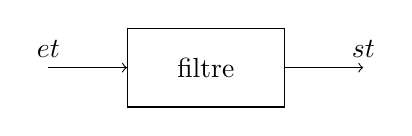
\begin{tikzpicture}
            \draw[->] (0, 0) node[above] {$e\p{t}$} -- (1, 0);
            
            \draw[] (1, -0.5) -- (1, 0.5) -- (3, 0.5) -- (3, -0.5) -- (1, -0.5);
            
            \node[] at (2, 0)  {filtre};
            
            \draw[->] (3, 0) -- (4, 0) node[above] {$s\p{t}$};
        \end{tikzpicture}
    \end{center}
    
    On supposera que les filtres étudiés sont linéaires, c'est-à-dire que $e\p{t}$ et $s\p{t}$ sont liés par une équation différentielle linéaire :
    %
    \[ \forall \lambda,\qquad \forall e_1, e_2 \ \text{ tels que } \ e_1 \rightarrow s_1 \et e_2 \rightarrow s_2,\qquad \lambda e_1 + e_2 \rightarrow \lambda s_1 + s_2\]
    
    \begin{example}{}{}
        Un même circuit électrique peut donner lieu plusieurs filtres :
        %
        \begin{center}
            \begin{circuitikz}
                \draw (0, 0) to[R, l=$R$] ++(2, 0) to[L, l=$L$] ++(2, 0) to[C, l=$C$, v=$u\p{t}$] ++(0, -2) to[short, i=$i\p{t}$] ++(-4, 0) to[open, v>=$e\p{t}$] ++(0, 2);
            \end{circuitikz}
        \end{center}
        
        \begin{enumerate}
            \itt Filtre 1 : $e\p{t} \rightarrow q\p{t}$
            %
            \[ L\dfrac{\dif^2 q}{\dif t^2} + R\dfrac{\dif q}{\dif t} + \dfrac{1}{C}q\p{t} = e\p{t}\]
            %
            \itt Filtre 2 : $e\p{t} = u\p{t}$
            %
            \[ LC\dfrac{\dif^2 u}{\dif t^2} + RC\dfrac{\dif u}{\dif t} + u\p{t} = e\p{t}\]
            %
            \itt Filtre 3 : $e\p{t} \rightarrow i\p{t}$ 
            %
            \[ L\dfrac{\dif i^2}{\dif t} + R\dfrac{\dif i}{\dif t} + \dfrac{1}{C}i\p{t} = \dfrac{\dif e}{\dif t}\]
        \end{enumerate}
    \end{example}
    
    Conséquence : en combinant la linéarité des filtres et la transformée de \textsc{Fourier}, on peut obtenir la réponse d'un filtre à une entrée périodique :
    %
    \[ e\p{t} = a_0 + a_1\cos{\omega t + \phi_1} + a_2\cos{2\omega t + \phi_2} + \dots \rightarrow b_0 + b_1\cos{\omega t + \varphi_1} + b_2\cos{2\omega t + \varphi_2} + \dots = s\p{t}\]
    
    On comprend donc l'importance de connaître la \underline{réponse harmonique} du filtre (l'effet du filtre sur une fonction sinusoïdale $e\p{t} = e_0\cos{n\omega t + \varphi}$). L'étude de cette réponse harmonique peut se faire grâce à la fonction de transfert $\underline{H}\p{j\omega}$ :

    Pour caractériser un filtre, on définit  $\underline{H}\p{j\omega} = \dfrac{\underline s}{\underline e}$ :
    %
    \[ e\p{t} = e \]
    
    \subsection{Filtre passe bas}
    
    \subsection{TODO}
    
    \newpage
    
    \subsection{Filtre passe haut}
    
    \subsubsection{Filtre passe haut idéal}
    
    \begin{center}
        \begin{tikzpicture}
            \begin{axis}[
                axis lines          =   center,
                domain              =   0:8,
                xlabel              =   $\omega$,
                ylabel              =   $G$,
                xmin                =   0,
                xmax                =   8,
                ymin                =   0,
                ymax                =   5,
                grid                = none,
                width               = 10cm,
                height              = 7cm,
                ytick               = {3},
                yticklabels         = {$H_0$},
                xtick               = {2},
                xticklabels         = {$\omega_b$},
                legend pos          = outer north east,
                legend style={row sep=0.1cm, font=\scriptsize}
            ]
                \addplot[color=main2,samples=51,smooth,thick,domain=2:8]{3};
                \legend{$G = \mod{H\p{\jj \omega}}$}
                
                \draw[color=main2,thick,domain=2:8] (0, 0) -- (2, 0) -- (2, 3);
            \end{axis}
        \end{tikzpicture}
    \end{center}
    
    \begin{enumerate}
        \itt Si $\omega \gg \omega_b$ pour un signal périodique, alors :
        %
        \[ e\p{t} = e_0 + e_\text{ond}\p{t} \rightarrow s\p{t} = H_0e_\text{ond}\p{t}  \]
        %
        La première utilité du filtre est donc d'éliminer la valeur moyenne.
    
        \itt Si $k\omega < \omega_b < \p{k+1}\omega$, alors :
        %
        \[ e\p{t} = e_0 + \sum_{n=1}^{+\infty} e_n\p{t} \rightarrow s\p{t} = H_0\sum_{n=k+1}^{+\infty} e_n\p{t}  \]
    \end{enumerate}
    
    On remarquera que si $k$ et grand seules les harmoniques de rang élevées sortent, $s\p{t}$ a ainsi la forme des discontinuités de $e\p{t}$ :
    
    
    \begin{minipage}{0.48\linewidth}
        \begin{center}
            \begin{tikzpicture}
                \draw[main2, thick] (0, 0) -- (1, 0) -- (1, 1) -- (2, 1) -- (2, 0) -- (3, 0) -- (3, 1) -- (4, 1) -- (4, 0) -- (5, 0);
            \end{tikzpicture}
        \end{center}
    \end{minipage}
    %
    \begin{minipage}{0.04\linewidth}
        \[ \rightarrow \]
    \end{minipage}
    %
    \begin{minipage}{0.48\linewidth}
        \begin{center}
            \begin{tikzpicture}
                \draw[main2, thick] (0, 0) -- (0.98, 0) -- (1, 1) -- (1.02, 0) -- (1.98, 0) -- (2, -1) -- (2.02, 0) -- (2.98, 0) -- (3, 1) -- (3.02, 0) -- (3.98, 0) -- (4, -1) -- (4.02, 0) -- (5, 0);
            \end{tikzpicture}
        \end{center}
    \end{minipage}
    
    \subsubsection{Passe haut du premier ordre}
    
    Un filtre passe haut du premier ordre a pour équation :
    %
    \[ \tau \dfrac{\dif s}{\dif t} + s = H_0\tau \dfrac{\dif e}{\dif t} \qquad\text{soit}\qquad H\p{\jj\omega} = \dfrac{H_0\jj \omega \tau}{1 + \jj\omega \tau}\]
    %
    On a donc le gain et la phase :
    %
    \[ G_\text{dB} = 20\log \dfrac{H_0\frac{\omega}{\omega_0} }{ \sqrt{1 + \p{\frac{\omega}{\omega_0}}^2}} \qquad \varphi = \dfrac{\pi}{2} - \arg{1 + \jj\omega t}\]
    
    DIAGRAMME DE BODE A AJOUTER
    
    \subsubsection{Comportement dérivateur d'un passe haut du premier ordre}
    
    \begin{definition}{Comportement dérivateur}{}
    %
    \[ s\p{t} = H_0\tau \dfrac{\dif e}{\dif t} \qquad\text{soit}\qquad H\p{\jj\omega} = H_0\jj\omega \tau\]
    \end{definition}
    
    Problème : un dérivateur pur amplifie les termes $\omega \to +\infty$, et sature donc le système.
    
    Pour résoudre ce problème, on peut utiliser un passe haut tel que $\omega_b \gg \omega_\text{utilisateur}$. Ainsi, toutes les premières harmoniques sont dérivées :
    %
    \[ s\p{t} \approx H_0\tau\dfrac{\dif e}{\dif t}\]
    
    \subsubsection{Passe haut du deuxième ordre}
    
    Un filtre passe haut du deuxième ordre a pour équation :
    %
    \[ \dfrac{1}{\omega_0^2} \dfrac{\dif^2 s}{\dif t^2} + \dfrac{2\sigma}{\omega_0}\dfrac{\dif s}{\dif t} + S = \dfrac{H_0}{\omega_0^2} \dfrac{\dif^2 e}{\dif t^2} \qquad\text{soit}\qquad H\p{\jj\omega} = \dfrac{-H_0\p{\frac{\omega}{\omega_0}}}{1 + 2\sigma\jj\frac{\omega}{\omega_0} - \p{\frac{\omega}{\omega_0}}^2} \]
    %
    DIAGRAMME DE BODE A AJOUTER
    
    On remarquera que si $\sigma > 1$, alors $H_\text{PH ordre 2} = H_{PH ordre 1, I}\times H_{PH ordre 1, II}$

    \subsection{Passe bande}
    
    \subsubsection{Définition et diagramme de Bode}
    
    \section{Numérisation et traitement numérique}
    
    \section{Portes logiques}
    
    En électronique analogique, on réalise des circuits qui créent des signaux variables qui prennent des valeurs dans tout $\bdR$. Les composants de ces circuits vieillissent et sont sensibles à la température et à l'humidité, ces facteurs structurels plus les bruits de mesure peuvent dégrader le signal au point de dénaturer l'information.
    
    L'électronique numérique utilise des circuits ou la seule grandeur utile est la tension qui est bivalente : Soit $0$ la tension de la masse, soit $V_\text{cc}$ la tension d'alimentation. On parle de niveaux logiques. Les circuits sont composés de composants élémentaires reliés par des fils conducteurs qui transmettent des tensions bivalentes. Les entrées et sorties de ces composants sont des variables logiques bivalentes.
    
    \subsection{Portes logiques et logique combinatoire}
    
    \subsubsection{Principe}
    
    \subsection{Logique séquentielle}
    
    \subsubsection{Définition, exemple de la bascule $RS$}
    
    Les circuits de logique combinatoire ont des sorties qui dépendent uniquement de l'état des entrées au même instant. Au contraire, les circuit de logique séquentielle sont tels que les sorties dépendent des entrées mais aussi des valeurs antérieures des sorties. Le temps devient une variable importante $s = f\p{e_1, e_2, \dots, t}$. Ce sont des circuit avec des boucles de rétroaction : la sortie est renvoyée vers l'entrée. Dans le cadre de la logique séquentielle, un même jeu d'entrée peut donner des sorties de valeurs différentes, selon l'état antérieur du circuit.
    
    \begin{definition}{Bascule $RS$}{}
        Un exemple basique de circuit séquentiel est la bascule $RS$ : c'est un circuit à deux entrées $R$ et $S$ et une sortie $Q$ :
        %
        \[ table de vérité \]
    \end{definition}
    %
    On peut représenter une bascule $RS$ de la manière suivante :
    %
    \begin{center}
        \begin{tikzpicture}
            
        \end{tikzpicture}
    \end{center}
    
    \chapter{Changements de référentiel et dynamique non galiléenne}
    
    Dans les cours de mécanique de première année, on s'est toujours placé dans le cadre d'un repère galiléen (sauf peut-être en devoir sur table). Cependant, les repères auxquels l'on est confronté dans la majorité des situations plus concrètes ne présentent pas cette caractéristique, ce qui rend l'étude mécanique d'un corps y évoluant bien plus compliquée. Pour palier cette difficulté, une solution consiste à considérer le mouvement de ces référentiels par rapport à un autre référentiel, lui galiléen. Par exemple, on sait déjà qu'un référentiel en translation uniforme par rapport à un référentiel galiléen est galiléen. Il s'agira donc dans ce chapitre d'étudier les mouvements des référentiels entre eux, et d'ainsi généraliser les lois de la mécanique étudiée en première année dans le cas non-galiléen.
    
    \chaptertoc
    
    \section{Référentiels}
    
    \subsection{Quelques considérations sur la mécanique (HP)}
    
    
    \emph{Ce paragraphe est inspiré de \emph{Notes pour l'étude du cours de Mécanique}, par \textsc{C. Marie} en \emph{1978-1979}.}\medskip
    
    Globalement, la mécanique est une science qui donne une schématisation mathématiques des corps dans l'espace au cours du temps. Elle est constitué de deux parties principales : la cinématique, qui permet de décrire rigoureusement et mathématiquement les objets étudiés, et la dynamique, qui offre une explication de ces mouvements en explicitant leur causes. Plusieurs fois dans l'histoire, les lois de la mécanique ont été changées, revues, voire totalement remplacées, pour rendre compte de la réalité avec divers degré de précisions et divers contextes.
    
    Aujourd'hui, on distingue notamment la mécanique classique (ou Newtonienne) qui étudie les objets macroscopiques de vitesse faible devant celle de la lumière, la mécanique relativiste (depuis \textsc{Einstein}) qui traite des cas plus généraux (notamment compatible avec la relativité restreinte et général, d'où le nom), et la mécanique quantique qui étudie les systèmes à l'échelle atomique et subatomique. Dans ce chapitre, on se placera toujours dans le cadre mécanique classique.\medskip
    
    Empiriquement, on constate que les phénomènes mécaniques ont lieu dans \guill{l'espace physique} et au cours du \guill{temps}. Le premier est intuitivement percu comme un continuum tridimensionnel et le second comme un continuum unidimensionnel et unidirectionnel (on a une \guill{flèche de temps} dirigée du passé vers l'avenir). Il n'y a \textit{a priori} aucune raison de supposer le temps comme cyclique, ni comme limité dans le passé ou dans le futur. De plus, l'existence de phénomènes physiques périodiques (par exemple la transition hyperfine de l'état fondamental de l'atome de césium 133 non perturbé, qui permet de définir la seconde) permet de graduer ce temps. Ainsi :
    %
    \begin{definition}{Temps}{}
        On appelle \hg{temps} le \hg{$\bdR$-espace affine} de \hg{dimension $1$}, 
    \end{definition}
    
    \subsection{Référentiels et repères}
    
    On commence par rappeler quelques définitions, notamment la notion de référentiel et de repère. Dans tout ce chapitre (et même généralement en physique), on considérera que l'espace de dimension $3$ est euclidien (en tout cas sur de courtes distances).
    
    \begin{definition}{Référentiel}{}
        Un \hg{référentiel} est le donnée d'un \hg{solide $\Sigma$} et d'une \hg{horloge}.
    \end{definition}
    
    Il ne faut pas confondre référentiel et repère. Un repère n'a pas de sens physique, et il ne s'agit que d'un outil mathématique.
    
    \begin{definition}{Repère}{}
        On appelle \hg{repère} la donnée d'\hg{un point}, appelé \hg{origine du repère}, et de \hg{trois vecteurs} linéairement indépendants.
    \end{definition}
    
    \begin{notation}
        Un repère \hg{$R$ d'origine $O$ et de vecteurs $\vec i, \vec j,\vec k$} sera généralement noté avec un $4$-uplet : $\hg{R = \p{O, \vec i, \vec j, \vec k}}$.
    \end{notation}
    
    L'objectif d'un repère est de se repérer dans l'espace. On a revu dans un chapitre précédent les exemples du repère cartésien, polaire, cylindrique, sphérique, \dots\newline
    
    Si l'on considère un référentiel $\bcR$ (dont le solide est bien de dimension 3), on peut déterminer un repère $R$ associé à $\bcR$ en choisissant quatre points $\p{O, A, B, C}$ de $\Sigma$ tels que $\vec{OA}$, $\vec{OB}$ et $\vec{OC}$ sont linéairement indépendants. $R = \p{O, \vec{OA}, \vec{OB}, \vec{OC}}$ est alors un repère associé à $\bcR$.
    
    \begin{enumerate}
        \itt On remarque bien qu'il y a une infinité de repères associables au référentiel $\bcR$. Cependant, par abus de langages, on confondra souvent $R$ et $\bcR$.
    \end{enumerate}
    
    \begin{example}{}{}
        On donne ci-dessous quelques exemples de repères  $R = \p{0, \vec i, \vec j, \vec k}$ :
        \begin{enumerate}
            \itt \hg{Référentiel de \textsc{Copernic}} : $O$ est le centre de gravité du système solaire et $\vec i, \vec j, \vec k$ pointent trois étoiles très lointaines.

            \itt \hg{Référentiel héliocentrique} : $O$ est le centre du soleil et $\vec i, \vec j, \vec k$ sont les mêmes que dans le repère de \textsc{Copernic}.
        
            \itt \hg{Référentiel géostationnaire} : $O$ est le centre de la Terre et $\vec i, \vec j, \vec k$ pointent vers les mêmes étoiles que dans les référentiels ci-dessus. 

            \itt \hg{Référentiel terrestre} : $O$ est le centre de la Terre et $\vec i, \vec j, \vec k$  sont liés à la Terre. 

            \itt \hg{Référentiel lié à un train} : $O$ est un point du train et $\vec i, \vec j, \vec k$ sont liés au train.
        \end{enumerate}
    \end{example}
    
    \subsection{Mouvement relatif entre deux référentiels}
    
    Dans cette partie, on prendra $\bcR_1$ et $\bcR_2$ auxquels on associe deux référentiels $R_1$ et $R_2$ (respectivement), tels que $R_1 = \p{O_1, \vec{i_1}, \vec{j_1}, \vec{k_1}}$ et $R_2 = \p{O_2, \vec{i_2}, \vec{j_2}, \vec{k_2}}$.
    
    \subsubsection{Mouvement de translation de $\bcR_2$ par rapport à $\bcR_1$}
    
    On commence par s'intéresser au mouvement de translation. Celui-ci se définit de la manière suivante :

    \begin{definition}{Translation}{}
        On dit que \hg{$\bcR_2$ est en translation par rapport à $\bcR_1$} lorsque :
        %
        \[ \hg{\forall M \in \bcR^3 \ \text{tel qu'à tout instant} \ t \ \text{on a} \  \vec{v_{\bcR_2}}\p{M} = 0, \exists \vec{cte}\p{t} \in \bdR^3,\qquad \forall M \in \bdR^3 \ \text{tel que} \ \vec{v_2}\p{M_2} = 0,\qquad \vec{v_1}\p{M_2, t} = \vec{cte}\p{t}}\]
    \end{definition}
    %
    Ce qui siginifie, moins formellement, que $\bcR_2$ est en translation par rapport à $\bcR_1$ lorsque tout point $M$ fixe dans $\bcR_2$ a le même vecteur vitesse dans $\bcR_1$. 
    %
    On obtient ainsi la propriété suivante :
    %
    \begin{property}{}{}
        Si \hg{$\bcR_2$ est en translation par rapport à $\bcR_1$}, alors :
        %
        \begin{psse}
            \itast \hg{Le mouvement de $\bcR_2$} dans $R_1$ \hg{est entièrement défini par $\vec{v_1}\p{O_2}$}.
            
            \itast \hg{Les axes de $R_2$ gardent une direction fixe} au cours du mouvement de $\bcR_2$.
        \end{psse}
    \end{property}
    
    On donne ci-dessous quelques exemples de mouvements de translation :

    \begin{example}{}{}
        \begin{enumerate}
            \itt \(R_2\)(Train) dans \(R_\text{terrestre} = R_1\). Sur une voie rectiligne \(R_2\) est 
            en translation par rapport à \(R_1\), si \(\vec{V_1}(O_2) = \vec{cte}(t) = \vec{cte}\) alors 
            la translation est rectiligne uniforme.

            \itt \(R_{\text{géostationnaire}}\) et \(R_\text{héliocentrique}\)
            % je sais pas faire les beaux dessins
            La translation est curviligne, \(O_2\) parcours une ellipse dans \(R_1\)
        \end{enumerate}
    \end{example}

    \subsubsection{Mouvement de rotation de $\bcR_2$ par rapport à $\bcR_1$}
    
    Cas particulier : mouvement de rotation autour d'un axe fixe \(\Delta\) de \(R_1\), on prend \(R_1\) tel que \(\Delta = (O_1, \vec{k_1})\), \(R_1 = (0_1, \vec{i_1}, \vec{j_1}, \vec{k_1})\). \\
    On peut donc choisir \(O_2 = O_1,\  \vec{k_2} = \vec{k_1}\) dans \(R_2 = (O_2, \vec{i_2}, \vec{j_2}, \vec{k_2})\). On retrouve alors le repère cylindrique où \(\vec{i_2} = \vec{u_r},\ \vec{j_2} = \vec{u_{\theta}}\) ainsi \(R_2 = (O_2, \vec{u_r}, \vec{u_{\theta}}, \vec{k_1})\) \newline

    On sait alors que l'on peut définir le vecteur rotation de \(R_2\) par rapport à \(R_1\) : \(\vec{\Omega}_{R_2/R_1} = \dot{\theta}\vec{k_1}\)

    \begin{definition}{Vecteur rotation}{}
        Le vecteur rotation de \(R_2\) dans \(R_1\) est tel que 
        \begin{enumerate}
            \itt \( \dfrac{d \vec{i_2}}{dt} = \vec{\Omega}_{R_2/R_1} \wedge \vec{i_2}\)

            \itt \( \dfrac{d \vec{j_2}}{dt} = \vec{\Omega}_{R_2/R_1} \wedge \vec{j_2}\)

            \itt \( \dfrac{d \vec{k_2}}{dt} = \vec{\Omega}_{R_2/R_1} \wedge \vec{k_2}\)
        \end{enumerate}
    \end{definition}
    
    \subsection{Mouvement le plus général}
    
    Le Mouvement le plus général de $\sfrac{\bcR_2}{\bcR_1}$ (de $\bcR_2$ par rapport à $\bcR_1$) est tangent à un mouvement hélicoïdal entièrement caractérisé par $\vec{v_1}\p{O_2}$ et $\vec{\bcM_{\sfrac{2}{1}}}$.
    
    \subsection{Dérivée covariante}
    
    On développe ici la formule de la dérivvée covariante (\ie. formule de la dérivation composée) :
    
    \begin{property}{Dérivée covariante}{}
        Soient deux \hg{référentiels $\bcR_1$} et \hg{$\bcR_2$} et un \hg{vecteur $\vec X$}. On a :
        %
        \[ \hg{\intc{\dfrac{\dif \vec X}{\dif t}}_{\bcR_1} = \intc{\dfrac{\dif \vec X}{\dif t}}_{\bcR_2} + \vec{\bcM_{\sfrac{\bcR_2}{\bcR_1}}} \land \vec{X}}\]
    \end{property}
    %
    \begin{nproof}
        Soient deux référentiels $\bcR_1$ et $\bcR_2$ de repères respectifs $R_1 = \p{O_1, \vec{i_1}, \vec{j_1}, \vec{k_1}}$ et $\p{O_2, \vec{i_2}, \vec{j_1}, \vec{k_2}}$, ainsi qu'un vecteur $\vec X$ tel que :
        %
        \[ \vec X = x_1 \vec{i_1} + y_1 \vec{j_1} + z_1 \vec{k_1}
        = x_2 \vec{i_2} + y_2 \vec{j_2} + z_2 \vec{k_2}\]
        %
        On cherche alors une relation entre $\intc{\dfrac{\dif \vec X}{\dif t}}_{\bcR_1}$ et $\intc{\dfrac{\dif \vec X}{\dif t}}_{\bcR_2}$ :
        %
        \[
            \intc{\dfrac{\dif \vec X}{\dif t}}_{\bcR_1} = \intc{\dfrac{\dif}{\dif t}\p{x_2\vec{i_2} + y_2\vec{j_2} + z_2\vec{k_2}}}_{\bcR_1} = \dot x_2\vec{i_2} + \dot y_2\vec{j_2} + \dot z_2\vec{k_2} + x_2\intc{\dfrac{\dif \vec{i_2}}{\dif t}}_{\bcR_1} + y_2\intc{\dfrac{\dif \vec{j_2}}{\dif t}}_{\bcR_1} + z_2\intc{\dfrac{\dif \vec{k_2}}{\dif t}}_{\bcR_1}
        \]
        %
        En notant $\bcM_{\sfrac{2}{1}}$ pour $\bcM_{\sfrac{\bcR_2}{\bcR_1}}$, On obtient alors :
        %
        \[ \intc{\dfrac{\dif \vec X}{\dif t}}_{\bcR_1} = \intc{\dfrac{\dif \vec X}{\dif t}}_{\bcR_2} + x_2 \vec{\bcM_{\sfrac{2}{1}}} \wedge \vec{i_2} + y_2 \vec{\bcM_{\sfrac{2}{1}}} \wedge \vec{j_2} + z_2 \vec{\bcM_{\sfrac{2}{1}}} \wedge \vec{k_2} = \intc{\dfrac{\dif \vec X}{\dif t}}_{\bcR_2} + \vec{\bcM_{\sfrac{2}{1}}} \wedge \p{x_2 \vec{i_2} + y_2 \vec{j_2} + z_2 \vec{k_2}}\]
        %
        Ce qui livre finalement le résultat attendu :
        %
        \[ \intc{\dfrac{\dif \vec X}{\dif t}}_{\bcR_1} = \intc{\dfrac{\dif \vec X}{\dif t}}_{\bcR_2} + \vec{\bcM_{\sfrac{\bcR_2}{\bcR_1}}} \land \vec{X}\]
    \end{nproof}

    
    \section{Loi de composition des vitesses}
    
    Dans cette section, on considérera de même $\bcR_1$ et $\bcR_2$ deux référentiels, de repères respectivement associés $R_1 = \p{O_1, \vec{i_1}, \vec{j_1}, \vec{k_1}}$ et $R_2 = \p{O_2, \vec{i_2}, \vec{j_2}, \vec{k_2}}$.
    
    On cherche à établir un lien entre $\vec{v_1}\p{M}$ et $\vec{v_2}\p{M}$, et également entre $\vec{a_1}\p{M}$ et $\vec{a_2}\p{M}$.
    
    Mouvement de $\bcR_1$ dans $\bcR_2$ est caractérisé par
    $\vec{V_1}\p{O_2}$ et $\Omega_{\bcR_2 / \bcR_1}$
    
    \subsection{Cas d'un référentiel $\bcR_2$ en translation par rapport à $\bcR_1$}
    
    Soient $R_1 = \p{O_1, \vec{i_1}, \vec{j_1}, \vec{k_1}}$ et $R_2 = \p{O_2, \vec{i_2}, \vec{j_2}, \vec{k_2}}$.
    
    \(\vec{V_1}\p{M} = \p{\frac{d\vec{O_1 M}}{dt}}_1
    \vec{V_2}\p{M} = \p{\frac{d\vec{O_2 M}}{dt}}_1\)
    
    $\vec{O_1 M} = \vec{O_1 O_2} + \vec{O_2 M}$
    
    $\vec{V_1} \p{M} = \p{\frac{d\vec{O_1 O_2}}{dt}}_1 + \p{\frac{d\vec{O_2 M}}{dt}}_1$
    
    $\vec{V_1}\p{M} = \vec{V_1}\p{O_2} + \p{\frac{d\vec{O_2 M}}{dt}}_2 + \vec{\Omega}_{2/1} \land \vec{O_2 M}$
    
    $\implies \vec{V_1} = \vec{V_1}\p{0_2} + \vec{V_2}\p{M}$
    
    On note (terminologie)
    \begin{enumerate}
        \itt $\vec{V_1}\p{M} = \vec{V_a}\p{M}$ vitesse absolue
        
        \itt $\vec{V_2}\p{M} = \vec{U_r}\p{M}$ vitesse relative
        
        \itt $\vec{V_1}\p{O_2} = \vec{V_e}\p{M}$ vitesse d'entraînement de $\bcR_2 \\ \bcR_1$ en M
    \end{enumerate}

    On remarquera deux choses :
    %
    \begin{enumerate}
        \itt Cette loi de composition des vitesses n'est valable qu'en mécanique classique, en relativité restreinte \(v_\text{max} = c\)

        \itt La vitesse d'entraînement apparaît comme la vitesse du point \(P\) coïncidant à \(M\) et fixe dans \(R_2\)
    \end{enumerate}

  \subsection{Loi de composition des accélérations}

    \begin{definition}{Accélérations composées}{}
        On a les accélérations dans les deux repères définies par :
        \[\vec A_1 = \left( \dfrac{\dif \vec V_1(M}{\dif t}\right)_1 \quad 
        \vec A_2 = \left( \dfrac{\dif \vec V_2(M}{\dif t}\right)_2\]

        Ainsi \( \vec A_1 = \left( \dfrac{\dif}{\dif t} \p{\vec V_1(O_2) + V_2(M )}\right)_1 = 
        \vec A_1(O_2) + \left(\dfrac{\dif \vec V_2(M}{\dif t}\right)_2 + \vec \Omega_{R_2/R_1} \wedge \vec V_2 = \vec A_2(M) + \vec A_1(O_2)\)
    \end{definition}
    
    \begin{example}{Ordre de grandeur}{}
        Soit $\bcR_2$ le référentiel terrestre et $\bcR_1$ le référentiel géocentrique, de même origine $O$. On cherche à calculer la vitesse $v_{e, \bcR_2 / \bcR_1}\p{P_\text{France}}$ d'un point $P_\text{France}$ (situé en France) de $\bcR_2$ dans $\bcR_1$. On a :
        %
        \[ v_{e, \bcR_2 / \bcR_1}\p{P_\text{France}} = \vec \bcM_{\bcR_2 / \bcR_1} \wedge \vec{O'M} = \bcM_{\bcR_2 / \bcR_1} \times O'M \times \sin{\theta} \vec{u_\theta} = HM \bcM_{\bcR_2 / \bcR_1} \vec{u_\theta}\]
        Application Numérique : $HM = R_T \sin{45°}$
        $\bcM_{\bcR_2 / \bcR_1} = \bcM_T = \frac{2 \pi}{\text{1 jour}} = \frac{2 \pi}{3 \cos{2 \pi}} = 7 \times 10^{-5} rad s^{-1}$
        $V_e (Mt France) = 1700 km h^{-1}$
    \end{example}
    
    \subsubsection{Loi de composition des accélérations}
    
    On a :
    %
    \[ \vec{a_{\bcR_1}}\p{M} = \intc{\dfrac{\dif^2 \vec{O_1M}}{\dif t}}_{\bcR_1} = \intc{\dfrac{\dif \vec{v_{\bcR_1}}\p{M}}{\dif t}}_{\bcR_1}\]
    %
    Et :
    %
    \[ \vec{a_{\bcR_2}}\p{M} = \intc{\dfrac{\dif^2 \vec{O_2M}}{\dif t}}_{\bcR_2} = \intc{\dfrac{\dif \vec{v_{\bcR_2}}\p{M}}{\dif t}}_{\bcR_2}\]
    %
    Ainsi :
    %
    \begin{align*}
        \vec{A_{\bcR_1}}\p{M} &= \intc{\dfrac{\dif \vec{V_{\bcR_2}\p{M}}}{\dif t}}_{\bcR_1} + \intc{\dfrac{\dif}{\dif t}\p{\vec \Omega_{\bcR_2/\bcR_1} \wedge \vec{O_2M}}}_{\bcR_1}\\
        &= \intc{\dfrac{\dif \vec{V_{\bcR_2}\p{M}}}{\dif t}}_{\bcR_1} + \vec \Omega_{\bcR_2/\bcR_1} \wedge \vec{V_{\bcR_2}\p{M}} + \underbrace{\intc{\dfrac{\dif \vec \Omega_{\bcR_2/\bcR_1}}{\dif t}}}_{\vec 0} \wedge \vec{O_2M} + \vec \Omega_{\bcR_2/\bcR_1} \wedge \intc{\dfrac{\dif \vec{O_2M}}{\dif t}}_{\bcR_1}\\
        &= \vec{a_{\bcR_2}}\p{M} + \vec \Omega_{\bcR_2/\bcR_1} \wedge \vec{v_{\bcR_2}}\p{M} + \vec{\bcM_{\bcR_2/\bcR_1}} \wedge \p{\intc{\dfrac{\dif \vec{O_2M}}{\dif t}}_{\bcR_2} + \vec \Omega_{\bcR_2/\bcR_1} \vec{O_2M}\p{t}}\\
        &= vec{A_{\bcR_2}}\p{M}
    \end{align*} 
    
    Donc on a finalement :
    %
    \[ \vec{a_{\bcR_1}}\p{M} = \vec{a_{\bcR_2}}\p{M} + 2\vec \Omega_{\bcR_2/\bcR_1} \wedge \vec{v_{\bcR_2}}\p{M} +  \bcM_{\bcR_2/\bcR_1} \wedge \p{ \bcM_{\bcR_2/\bcR_1} \wedge \vec{O_2M}}\]
    
    On peut voir la formule de la façon suivante :
    %
    \[ \vec{A_a} = \vec{A_r} + \vec{A_C}\p{M} + \vec{A_e}\p{M}\]
    %
    \begin{enumerate}
        \itt $\vec{A_a}$ est l'accélération \guill{absolue} dans $\bcR_1$
        
        \itt $\vec{A_r}$ est l'accélération \guill{relative} dans $\bcR_2$
        
        \itt $\vec{A_e}$ est l'accélération \guill{d'entraînement}
        
        \itt $\vec{A_C}$ est l'accélération de \textsc{Coriolis} :
    \end{enumerate}
    
    \begin{definition}{Accélération de Coriolis}{}
        Soient deux repères $\bcR_1$ et $\bcR_2$, l'accélération de \textsc{Coriolis} de $M$ dans $\bcR_1$ par rapport à $\bcR_2$ est :
        %
        \[ \hg{\vec{A_C}\p{M} = 2\vec \Omega_{\bcR_2/\bcR_1} \wedge \vec{V_{\bcR_2}}\p{M}}\]
    \end{definition}
    
    (A recopier)
    
    \newpage
    
    \begin{form}{A retenir}{}
        \begin{enumerate}
            \itt Formule de la \hg{dérivée covariante} :
            %
            \[ \hg{\intc{\dfrac{\dif \vec X}{\dif t}}_{\bcR_1} = \intc{\dfrac{\dif \vec X}{\dif t}}_{\bcR_2} + \vec \Omega_{\bcR_2 / \bcR_1} \wedge \vec{ X}}\]
            %
            \itt Lorsque \hg{$\bcR_2$ est en translation par rapport à $\bcR_1$} :
            %
            \begin{enumerate}
                \itast $\hg{\vec{V_{\bcR_1}}\p{M} = \vec{V_{\bcR_2}}\p{M} + \vec{V_e}\p{M}}$ où $\hg{\vec{V_e}\p{M} = \vec{V_{\bcR_1}}\p{O_2}}$.
                
                \itast $\hg{\vec{A_{\bcR_1}}\p{M} = \vec{A_{\bcR_2}}\p{M} + \vec{A_C}\p{M} + \vec{A_e}\p{M}}$ où $\hg{\vec{A_C}\p{M} = \vec 0}$. et $\hg{\vec{A_e}\p{M} = \vec{A_{\bcR_1}}\p{O_2}}$.
            \end{enumerate}
            
            \itt Lorsque \hg{$\bcR_2$ est en rotation uniforme autour d'un axe fixe de $\bcR_1$} (donc $O_1 = O_2$ fixe) :
            %
            \begin{enumerate}
                \itast $\hg{\vec{V_{\bcR_1}}\p{M} = \vec{V_{\bcR_2}}\p{M} + \vec{V_e}\p{M}}$ où $\hg{\vec{V_e}\p{M} = \vec\Omega_{\bcR_2/\bcR_1} \wedge \vec{O_2M}}$.
                
                \itast $\hg{\vec{A_{\bcR_1}}\p{M} = \vec{A_{\bcR_2}}\p{M} + \vec{A_C}\p{M} + \vec{A_e}\p{M}}$ où $\left\lbrace\begin{array}{l}
                    \hg{\vec{A_C}\p{M} = 2\vec\Omega_{\bcR_2/\bcR_1} \wedge \vec{V_{\bcR_2}}\p{M}} \\
                    \hg{\vec{A_e}\p{M} = \vec\Omega_{\bcR_2/\bcR_1} \wedge \p{\vec\Omega_{\bcR_2/\bcR_1} \wedge \vec{O_2M}}}
                \end{array}\right. $.
            \end{enumerate}
        \end{enumerate}
    
    \end{form}
        
    \section{Dynamique non-galiléenne}
    
    On s'intéresse maintenant à la dynamique en général, et on cherche à généraliser la dynamique de première année (uniquement dans les référentiels galéliens) à des référentiels quelconques en général. Il s'agira d'étudier les conditions et le coût de cette généralisation.
    
    \subsection{Référentiels galiléens}
    
    \subsubsection{Définitions}
    \begin{definition}{Référentiel galiléen}{}
    Un référentiel galiléen est galiléen si les lois de la mécanique Newtonienne s'appliquent.
    \end{definition}
    
    On remarque qu'un référentiel est galiléen si un système isolé dans ce référentiel a un mouvement rectiligne uniforme.
    
    \begin{property}{}{}
        Un référentiel en translation rectiligne uniforme par rapport à un référentiel galiléen est un référentiel galiléen.
    \end{property}

    \subsubsection{Caractère galiléen approché d'un référentiel}
    
    \begin{property}{Condition d'assimilation à un référentiel galiléen}{}
        Soient \hg{$\bcR_1$ et $\bcR_2$ deux référentiels}, et\hg{$\tau_\text{exp}$ le temps caractéristique} de l'étude. Si
        %
        \begin{enumerate}
            \itast \hg{$\bcR_1$ est un référentiel galiléen} ;
            \itast \hg{$\vec v\p{O'} \approx \vec{\text{cte}}$} ;
            \itast \hg{$\norm{\vec\Omega_{\bcR_2/\bcR_1}} \times \tau_\text{exp} \ll 2\pi$}
        \end{enumerate}
        %
        alors \hg{on assimilera $\bcR_2$ à un référentiel galiléen}.
    \end{property}

    
    
    
    %
    \begin{enumerate}
        \itt si $\tau_\text{exp} << 1 an$
        $\mod{\vec{V}\p{O_{Terre}}} \times \tau_\text{exp} << R_{TS}$
        $\implies si T_{exp} << 1 an alors \bcR_{géo} \equiv galilléen$
        \itt si $\tau_\text{exp} << 1 jour$
        $\implies si T_{exp} << 1 jour alors \bcR_{terrestre} \equiv galilléen$
    \end{enumerate}
    
    \subsubsection{Généralisation}
    
    Soit $\bcR_2$ et $\bcR_1$ avec $\bcR_1$ galiléen.
    
    PFD dans $\bcR_1$ : $m\vec{A_a}\p{M} = \sum \vec{F_\text{ext}}$.
    
    Or $\vec{A_a} = \vec{A_r}\p{M} + \vec{A_C}\p{M} + \vec{A_e}\p{M}$, d'où :
    %
    \[ m\vec{A_r}\p{M} = \sum \vec{F_\text{ext}} - m\vec{A_c}\p{M} - m\vec{A_e}\p{M}\]
    %
    On pose alors :
    %
    \begin{enumerate}
        \itt $\vec{F_{iC}} = -m\vec{A_C}\p{M}$ la force de \textsf{Coriolis}
        
        \itt $\vec{F_{ie}} = -m\vec{A_e}\p{M}$ la force d'entrainement
        
        \itt Les forces $\vec{F_{iC}}$ et $\vec{F_{ie}}$ sont dites forces d'inerties.
    \end{enumerate}
    
    \subsection{Loi de la dynamique du point matériel en référentiel non galiléen}
    
    \begin{form}{}{}
        \begin{enumerate}
            \itt Le \hg{principe fondamental de la dynamique} s'énonce :
            %
            \[ \hg{m\vec{A_r}\p{M} = \sum \vec{F_\text{ext}} + \vec{F_{iC}} + \vec{F_{ie}}}\]
            
            \itt Le \hg{théorème du moment cinétique} s'énonce :
            %
            \[ \hg{\intc{\dfrac{\dif \vec{\sigma_r}\p{M_2}}{\dif t}}_{\bcR_2} = \sum \vec{M_\text{ext}}\p{O_2} + \vec{\bcM_{F_{iC}}}\p{O_2} + \vec{\bcM_\text{fixe}}\p{O_2}} \]
            
            \itt Le \hg{théorème de l'énergie cinétique} s'énonce :
            %
            \[ \hg{\intc{\dfrac{\dif {E_c}_{\bcR_2}}{\dif t}}_{\bcR_2} = \sum \hg{\bcP_{c} + \bcP_{nc}} + \bcP_{iC} + \bcP_{ie}}\]
            %
            \itt Le \hg{théorème de l'énéergie mécanique} s'énnonce :
            %
            \[ \hg{\intc{\dfrac{\dif {E_m}_{\bcR_2}}{\dif t}} = \sum \bcP_{nc} + \bcP_{iC} + \bcP_{ie}}\]
        \end{enumerate}
    \end{form}
    
    En conclusion, on peut appliquer les lois de la mécanique dans un référentiel non-galiléen à condition d'ajouter les termes de Coriolis et d'entrainement.
    
    Remarques :
    \begin{enumerate}
        \itt Dans un exo de changement de référentiel ou de dynamique non galilléenne on commence par définir R2 et R1 et caractériser leurs mouvements relatifs
    \end{enumerate}
    
    \subsection{Expression des forces d'inerties et exemples}
    
    \subsubsection{Cas de $\bcR_2$ en translation par rapport à $\bcR_1$}

    %\begin{form}{Cas de \(R'\) en translation par rapport à \(R\)}{}
    %    \begin{enumerate}
    %        \itt On a \(R = \left(O,\vec e_x, \vec e_y, \vec e_z \right)\) et \(R' = \left(O', \vec e_x, \vec e_y, \vec e_z\right)\) 

    %        \itt On a donc \(\vec v_{e_{R'/R}}(M) = \vec v_R(O')\) ainsi que \(\vec A_{ic}=\vec 0\) et \(\vec A_{e_{R'/R}}(M) = \vec A_R(O')\) qui livrent 

    %        \[ \vec F_{ic} = \vec 0 \quad F_{ie} = -m\vec A_R(O')\]
    %        
    %    \end{enumerate}
    %\end{form}
    
    %\begin{example}{}{}
    %    \begin{enumerate}
    %        \itt Methode PFD :
    %            On considère le mouvement d'un pendule lors du démarrage d'une voiture.
    %        \(m\) est à l'équilibre relatif dans le repère \(R'\) de la voiture, on %applique donc le PFD dans \(R'\) projeté sur \(u_{\theta}\).
    %
    %        \[0 = 0 + ma_0\cos\theta + mg\sin\theta\]
    %
    %        Ainsi \(\theta_{eq} = \arctan\left(\dfrac{a_0}{g}\right)\)
    %
    %        \itt Méthode énergétique :
    %        %
    %        %\[ \delta W_F' = 0 \qquad\text{car}\qquad F \cdot \dif \vec{OM} = 0 = - %\dif E_{P_\vec T} \qquad\text{avec} \ E_{P_\vec T} = \text{cte} \]
    %    \end{enumerate}
    %\end{example}
    
    Deuxième exemple :
    %
    \begin{example}{Nacelle}{}
        %Dessin 
        La force d'inertie s'écrit $\vec{F_{ie}} = -m\vec{A_{ie}}\p{M}$.
    \end{example}
    
    \subsubsection{Cas de $\bcR_2$ en rotation uniforme autour d'un axe fixe de $\bcR_1$}

    \[\vec A_{ic}(M) = 2 \omega\vec e_z \wedge \vec v'(M) \quad \vec A_{ie}(M) = \vec\Omega_{R'/R} \wedge \left(\vec\Omega_{R'/R} \wedge \vec{O'M} \right) = \omega\vec e_z \wedge (\Omega\vec e_z \wedge \vec{OM}) = - \vec{HM} \omega^2 \]
    \begin{center}Ainsi on a\end{center} \[ F_{ie} + m \vec{HM} \omega^2 \quad F_{ic} = -2m \omega \vec e_z \wedge \vec v'(M)\]

    On remarquera que :
    %nul tes trucs ( no offense) (non ça épure rien)
    \begin{enumerate}
        \itt \(\vec F_{ie} = \vec 0\) sur l'axe
        \itt \(\vec F_{ie} \cdot \vec v_{R_2} > 0\) c'est ce qu'on appelle la force centrifuge.
    \end{enumerate}

    \begin{example}{}{}
        %enjoy dessiner le mec penché

        On prend \(R\) le référentiel terrestre supposé galiléen pour la durée de l'expérience et \(R'\) le référentiel lié au manège, en rotation. On se demande si l'on peut se pencher vers l'extérieur du manège sans tomber.

        On ayant les  frottements aussi grands qu'on veut, on peut avoir la somme des forces nulles mais 
        \[\sum \vec\bcM(P_0) = 0 + 0 + \vec\bcM_{\vec F_{ie}}(P_0) + \vec\bcM_{\vec F_{ic}}(P_0) \neq 0\]
        Le système n'a donc pas d'équilibre possible.
    \end{example}
    
    \subsection{Effet du caractère non galilléen du référentiel terrestre}

    On suppose que le référentiel géocentrique peut être supposé galiléen et le référentiel terrestre \(\bcR_T\) est en rotation autour de \(O_{\vec{e_z}}\)  l'axe des pôles à la vitesse angulaire \(\Omega_T = \frac{2\pi}{86400} = \SI{7.3e-5}{rad \cdot \second^{-1}}\)

    %enjoy le schéma des flèches autour de la terre
    \subsubsection{Effet de la force centrifuge}

    La Terre est une éllipsoïde donc \(\vec F_{ie} = m \vec{HM}\omega^2\) et \(\vec g = \vec G - \vec a_{ie}\)

    On remarquera que 
    \begin{enumerate}
        \itt La verticale définie par \(\vec g\) ne passe pas parle centre de la Terre si on ne se trouve ni aux pôles ni à l'équateur.

        \itt Dans un exercice de changement de référentiel sur Terre, on utilise \(\vec g\) donc pas besoin de calculer \(\vec F_{ie}\)

        \itt L'effet de marée est lié à \(\vec a_{ie}\) donc complicado que mucho

        \itt Effet de la force de Coriolis sur un repère local lié au référentiel terrestre
        % je laisse remy faire le  joli dessin
    \end{enumerate}

    \chapter{Le frottement solide}
    
    Ce chapitre étudie les frottements entre deux solides.
    
    \chaptertoc
    
    \section{Contact entre deux solides}
    
    Dans cette partie, on cherchera à étudier le contact entre deux solides
    $\Sigma_1$ et $\Sigma_2$. On traitera d'abord le cas où l'on peut
    modéliser la \guill{zone} de contact entre $\Sigma_1$ et $\Sigma_2$ par
    un point.
    
    \subsection{Contact ponctuel}
    
    \begin{minipage}{0.48\linewidth}
        DESSIN
    \end{minipage}
    %
    \hfill
    %
    \begin{minipage}{0.48\linewidth}
        On considère donc deux solides $\Sigma_1 \subset \bdR^3$ et $\Sigma_2 \subset \bdR^3$ dans l'espace. 
        %         
        \begin{enumerate}
            \itt $I$ est le point géométrique de contact entre $\ell_1$ et $\ell_2$. 
            
            \itt $I_1 \in \varphi_1$ confondu avec $I$
            
            \itt $I_2 \in \varphi_2$ confondu avec $I$
        \end{enumerate}
    \end{minipage}
    
    On définit trois référentiels : $\bcR$ le référentiel d'étude, $\bcR_1$ le référentiel lié à $\varphi_1$ et $\bcR_2$ le référentiel lié à $\varphi_2$. De plus, $\pi$ désigne le plan tangent aux $2$ solides en $I$.
    
    \begin{warning}{}{}
        On a les vitesses \hg{$\vec{v_1}\p{I_1} = \vec 0$} et \hg{$\vec{v_2}\p{I_2} = \vec 0$}. Cependant on peut aussi avoir :
        %
        \[ \hg{\vec v\p{I} \neq \vec v\p{I_1} \neq \vec v\p{I_2}}\]
    \end{warning}
    %
    Un exemple de ce principe est donné ci-dessous l'exemple d'une roue qui glisse vers l'avant :
    %
    \begin{example}{}{}
        \begin{minipage}{0.48\linewidth}
            \centering
            \begin{tikzpicture}
                \draw (0, 0) -- (3, 0);
                
                \node (G) at (1, 0.5) {G};
                \draw[-Latex, main3] (G) -- (2.5, 0.5) node[midway,label={[font=\footnotesize]$v_G$}] {};
                
                \node[draw,circle,minimum size=1cm] at (1,0.5) {};
            \end{tikzpicture}
        \end{minipage}
        %
        \begin{minipage}{0.48\linewidth}
            On a \hg{$\vec v\p{I \in \text{Sol}} = \vec 0$}, alors que \hg{$\vec v\p{I} = \vec v\p{G}$}.
        \end{minipage}
    \end{example}
    
    \subsubsection{Liaison plan-plan}
    
    Si la surface de contact entre deux solides est de dimension faible devant la longueur caractéristique du problème :
    %
    \[ \sqrt{s} \ll L_\text c \qquad\text{on supposera que le contact est ponctuel}\]
    %
    Dans les cas où le contact ne peut pas être assimilé à un contact ponctuel, on admet que tout se passe comme s'il était ponctuel en un point d'application $I$ :
    %
    \begin{center}
        \begin{tikzpicture}
            \draw (0, 0) -- (5, 0) -- (5, 2) -- (0, 2) -- (0, 0);
            \draw (2.5, 2) -- (4.5, 2) -- (4.5, 4) -- (2.5, 4) -- (2.5, 2);
            
            \node () at (7.5, 2) {$\iff$};
            
            \draw (10, 0) -- (15, 0) -- (15, 2) -- (10, 2) -- (10, 0);
            \draw (12.5, 2) -- (14.5, 2) -- (14.5, 4) -- (12.5, 4) -- (12.5, 2);
        \end{tikzpicture}
    \end{center}
    %
    Dans ce cas, la position de $I$ n'est pas forcément évidente, et il faut la déterminer. Pour cela :
    %
    \begin{enumerate}
        \itt On peut déterminer $I$ tel que $\vec{\bcM_\text{réel}}\p{I} = \vec 0$.
        
        \itt On peut aussi définir la position de $I$ pour qu'il n'y ait pas de rotation.
    \end{enumerate}
    
    \subsection{Glissement au contact entre deux solides}
    
    Soient deux solides $\varphi_1$ et $\varphi_2$, en contact ponctuel en $I$.
    %
    \begin{definition}{Vitesse de glissement}
        On appelle \hg{vitesse de glissement} la vitesse \hg{$\vec{v_g\p{\sfrac{\varphi_2}{\varphi_1}}} = \vec{g\sfrac{2}{1}}$}.
    \end{definition}
    

    \subsubsection{liaison parfaite}
    
        \begin{definition}{Liaison parfaite}{}
            Une liaison est dite parfaite si quel que soit le mouvement permis par la liaison, la puissance des actions de contact est nulle
        \end{definition}
    
        \begin{enumerate}
            \itt Liaison plan-plan parfaite : on a \( P_{c_{tot}} = P_{c_{12}} = \vec T_{1\to 2} \cdot \vec V_{g,2/1}\) or la liaison est parfait donc \(P_{c_{tot}} = 0\) donc même si \(\vec V_{g,2/1} \neq \vec 0\) on a \(\vec T_{1\to 2} = \vec 0\). Donc si la liaison plan-plan est parfaite il n'y a pas de frottements
    
            \itt Liaison pivot (nécessaire pour la rotation autour d'un axe fixe) %je te laisse faire les schémas, en gros c'est une truc qui tourne autour d'un axe (huile c pour qu'il y a pas de frottement)
            Par symétrie on a \(\vec T_{huile \to\Delta} = \vec 0\) et \[\vec \bcM_{\vec T}(O) = \int_0^{2\pi} \vec{OM} \wedge \dif \vec f = -\bbC \vec{u_{\Delta}} = - \alpha \Omega\vec u_{\delta}\] pour des frottements visqueux. Le moment est non nul à priori. \\ Si la liaison pivot est parfaite alors les actions de contacts ne travaillent pas, or pour une liaison pivot \(P_{c} = \vec \bbC\cdot \Omega\) où \(\bbC\) est le moment du couple, ainsi \(\vec \bbC = \vec 0 \Rightarrow\) pas de frottements.
        \end{enumerate}

    \section{Lois phénoménologiques}

    On s'interesse aux lois sur le frottement de glissement %aucune idée de ce que c'est mais wola c'est écrit au tableau 
    et donc aux Lois de \textsc{Coulomb} %xD il a découvert l'amerique xD xD xD

    \subsection{Expérience préliminaire}
        On suppose une caisse en liaison plan-plan avec le sol % je laisse faire le schéma
    
        \begin{center} %je te laisse faire le reste, tu comprends l'idée
            \begin{tikzpicture}
                \draw (0, 2) -- (5, 2);
                \draw (1.5, 2) -- (3.5, 2) -- (3.5, 4) -- (1.5, 4) -- (1.5, 2);
            \end{tikzpicture}
        \end{center}

    \subsection{Lois de Coulomb}

        \begin{enumerate}
            \itt S'il n'y a pas de glissements : \(\vec V_{g,2/1} = \vec 0\) alors \( || \vec T_{1\to 2} || \leq \mu_s || \vec N_{1\to 2} ||\)

            \itt s'il y a glissements : \(\vec V_{g,2/1} \neq \vec 0\) alors \( || \vec T_{1\to 2} || \leq \mu_d || \vec N_{1\to 2} ||\)
            
        \end{enumerate}

    \subsection{Propriétés des coefficients de frottements}

        \subsubsection{Ordre de grandeur (\(\mu_s \equiv \mu_d\))}

            \begin{enumerate}
                \itt métal-métal : \(0.1 \equiv 0.2\)
                \itt bois-bois : \(0;3 \equiv 0.4\)
                \itt papier-papier : \(0.5\)
                \itt pneu-bitume : \(0.5 \equiv 0.6\)
            \end{enumerate}

        \subsubsection{\(\mu\) est a priori une constante}
            On estime qu'elle ne dépend que du matériau de contact même si en réalité il y a une dépendance sur la vitesse.

        \subsubsection{\(\mu_d \equiv \mu_s\)}
            Sauf indication contraire on supposera toujours ces deux valeurs égales. Cependant l'écart entre les deux explique certains phénomènes tels que la craie qui crisse, le gond qui grince, ce sont des phénomènes dits de "collé-glissé"

        \subsection{Mesure de \(\mu\)}
            On considère un objet \(m\) sur un plan incliné d'angle \(\alpha\), \(\mu_s\) est la tangente de l'angle minimal tel que l'objet se met en mouvement.

    \section{Application}

        On considère l'exemple de la roue motrice %je te laisse faire le schéma
        \subsection{Hypothèse 1 : sans glissement}

            \[\vec V_{g,roue/sol} = \vec 0 = \vec V(I \in roue) = - \vec V\left( I \in sol\right)\]
            On a alors \(\vec V\left(I \in roue\right) = \vec 0\). Soir \(\bcR\) le référentiel du sol et \(\bcR_G\) le référentiel de la roue, on a alors \(\bcR_G\) est en translation par rapport à \(\bcR\) centrée en \(\bcG\). On a donc trivialement \(\vec V_R(I \in roue) = -R \omega \vec e_x + \dot{x} \vec e_x = (\dot{x} - R\omega)\vec e_x\) et on est sans glissement \(\dot x = R\omega\).

            Donc en appliquant le TMC en \(G\) dans \(\bcR_G\) en projection :
            \[ \dfrac{\dif \vec\sigma(G)}{\dif t} = \vec \bcM_T(G) + \vec \bcM_N(G) + \vec \bbC + \vec \bcM_{Fic}(G) + \vec \bcM_{Fie}(G) + \vec \bcM_{liaison}(G)\] donc on a trois équations après avoir projeté: \(J_{\Delta} \dot\omega = -RT+C \quad m\dot\dot x = T\quad \dot x = R\omega\)
            
    \chapter{Chimie en solution organique}
    
    Dans ce premier chapitre de physique, on étudiera surtout des solutés en solution aqueuse. On notera que de l'huile par exemple, n'est pas un soluté dans l'eau (on a deux phases distinctes). Par soluté, on entendra plutôt des entités comme des ions \emph{- le sel par exemple est $\p{Na^+, Cl^-}$ -}.
    
    \chaptertoc
    
    \section{La réaction chimique}
    
    \subsection{Introduction}
    
    \subsubsection{Notion de transformation}
    
    \begin{example}{Changement d'état du corps pur}{}
        \begin{center}
            \begin{tikzpicture}
                \node[rectangle,inner sep=7pt] (G) at (0, 3) {\phantom{\large Vapeur / Gaz}};
                \node[rectangle,inner sep=7pt] (S) at (-2.9, -1.5) {\phantom{\large Solide}};
                \node[rectangle,inner sep=7pt] (L) at (2.9, -1.5) {\phantom{\large Liquide}};
        
                \node[rectangle,fill=main4!50,opacity=0.5] at (0, 3) {\phantom{\large Vapeur / Gaz}};
                \node[rectangle,fill=main7!50,opacity=0.5] at (-2.9, -1.5) {\phantom{\large  Solide}};
                \node[rectangle,fill=main1!50,opacity=0.5] at (2.9, -1.5) {\phantom{\large Liquide}};
        
                \node[rectangle] at (0, 3) {\large\color{main4} Vapeur / Gaz};
                \node[rectangle] at (-2.9, -1.5) {\large\color{main7} Solide};
                \node[rectangle] at (2.9, -1.5) {\large\color{main1} Liquide};
        
                \draw[gradientdraw={0.3pt}{main4}{main7}, ->, main7] ([yshift=-4pt]G.west) to [bend left=20] node [sloped, anchor=center, below] {Condensation} (S.north);
        
                \draw[gradientdraw={0.3pt}{main7}{main4}, ->, main4] ([xshift=-4pt]S.north) to [bend left=20] node [sloped, anchor=center, above] {Sublimation} (G.west);
        
                \draw[gradientdraw={0.3pt}{main7}{main1}, ->, main1] ([yshift=-4pt]S.east) to [bend right=20] node [sloped, anchor=center, below] {Fusion} (L.west);
        
                \draw[gradientdraw={0.3pt}{main1}{main7}, ->, main7] ([yshift=4pt]L.west) to [bend right=20] node [sloped, anchor=center, above] {Solidification} (S.east);
        
                \draw[gradientdraw={0.3pt}{main1}{main4}, ->, main4] ([xshift=4pt]L.north) to [bend right=20] node [sloped, anchor=center, above] {Vaporisation} (G.east);
        
                \draw[gradientdraw={0.3pt}{main4}{main1}, ->, main1] ([yshift=-4pt]G.east) to [bend right=20] node [sloped, anchor=center, below] {Liquéfaction} (L.north);
            \end{tikzpicture}
        \end{center}
    \end{example}
    
    \begin{example}{Autres exemples}{}
        \begin{enumerate}
            \itt La distillation (mélange de deux liquides miscibles)
            
            \itt Changement de phase en crystallographie, par exemple :
            %
            \[ \mathrm{Fe}_\alpha \rightleftharpoons \mathrm{Fe}_\gamma \qquad\qquad\qquad C_\text{graphite} \rightleftharpoons C_\text{diamant} \]
            
            \itt transformations nucléaires  : réaction a l'intérieur des atomes qui ne restent pas identiques à eux mêmes, par exemple avec la radioactivité $\alpha$ : \quad on note $X_Z^A$ avec $Z$ le numéro atomique = nombre de protons et $A$ le nombre de masse = nombre de nucléons (protons et neutrons). :
            %
            \[ \mathrm X_Z^A \longrightarrow \mathrm Y_{Z-2}^{A-4} + \mathrm{Fe}_2^4 + \dots\]
            %
        \end{enumerate}
    \end{example}
    
    Les transformations chimique correspondent à un ré-arrangement des atomes entre eux par destruction de liaisons et constitution de nouvelles liaisons Il y a les mêmes atomes initialement et à la fin mais constituant des molécules différentes.

    \begin{example}{Réaction chimique}{}
        %
        \[ \ce{CH4_{(g)} + 2O2_{(g)} -> CO2_{(g)} + 2H2O_{(g)}} \]
        %
        On a à gauche $1$ atome de $C$, $4$ atomes de $H$ et $4$ atomes de $O$, et de même à droite.
    \end{example}
    
    \subsubsection{Grandeurs intensives de la composition d'une phase}
    
    On décrit quantitativement la composition d'un système chimique à l'aide de quantité de matière de chaque constituant.
    %
    \[ n_i = \text{nombre de mole du constituant} \]
    %
    On rappelle que :
    %
    \begin{enumerate}
        \itt $1$ mole correspond à $\bcN_A = \qty{6.02e23}{}$ entité identique.
        
        \itt $n_i = \dfrac{m_i}{M_i}$
    \end{enumerate}
    %
    On définit des variables intensives suivantes :
    \begin{enumerate}
        \itt En solution aqueuse pour un corps $A_i$ on définit sa concentration molaire :
        %
        \[ C_i = [A_i] = \frac{n_i}{V_i}\]
        %
        $V$ étant le volume du système étudié. $C_i$ s'exprime usuellement en \unit{\mol\per\litre}
        
        \itt On définit la fonction molaire de l'espèce $A_i$ dans un système par :
        %
        \[ x_i = \frac{n_i}{n_T} \]
        %
        avec $n_i = n\p{A_i}$ le nombre de mole de $A_i$ et $n_T = \displaystyle\sum_i n_i$ le nombre de mole total pensant dans le système.
    \end{enumerate}

    \begin{definition}{Pression partielle}{}
        On considère un gaz parfait $i$ occupant un volume $V$ à une température $T$, avec une quantité de matière $n_i$. On appelle \hg{pression partielle} la pression $P_i$ qu'aurait le gaz s'il était seul dans le même volume à la même température :
        %
        \[ \hg{P_i = \dfrac{n_iRT}{V}}\]
    \end{definition}
    %
    \begin{property}{Loi de Dalton}{}
        On a :
        %
        \[ \hg{\sum P_i = \dfrac{\p{\sum n_i}RT}{V} = \dfrac{n_\text tRT}{V} = P_\text t} \qquad\text{donc}\qquad \hg{P_\text t = \sum P_i}\]
        %
        \[ \hg{\dfrac{P_i}{P_\text t} = \dfrac{\frac{n_iRT}{V}}{\frac{n_\text t RT}{V}} = \dfrac{n_i}{n_\text T} = x_i} \qquad\text{donc}\qquad \hg{P_i = x_iP_\text t}\]
    \end{property}
    
    \subsection{La réaction chimique}
    \subsubsection{Description de la réaction chimique}
    
    \begin{center}
        \emph{Vocabulaire et notation}
    \end{center}
    %
    La transformation chimique de $A$ et $B$ donnant $C$ et $D$ est représenté par une écriture formelle de la réaction chimique qui tient compte des \emph{proportions} qui réagissent.
    %
    \[ \alpha A + \beta B \rightleftharpoons \gamma C + \delta D \]
    %
    \begin{enumerate}
        \itt $A$ et $B$ sont les \emph{réactifs}
        \itt $C$ et $D$ sont les \emph{produits}
        \itt $\rightharpoonup$ est le sens direct
        \itt $\leftharpoondown$ est le sens inverse
        \itt $\alpha$, $\beta$, $\gamma$ et $\delta$ sont les \emph{coefficients st\oe{}chiométriques} de $A$, $B$, $C$ et $D$ respectivement).
    \end{enumerate}
    
    
    \begin{property}{}{}
        \begin{enumerate}
            \itt conservation de la matières : les atomes présents dans les réactifs se retrouvent dans les produits.
            \itt conservation de la charge : le nombre total de charges des réactifs est égale à celui des produits
        \end{enumerate}
    \end{property}
    
    Ces 2 propriétés servent à écrire à écrire les réactions chimiques. Quand on connaît les espèces réactifs et produits.
    
    \begin{center}
        \emph{Coefficients stoechiométriques algébriques}
    \end{center}
    
    $\nu_i$ est le coefficient st\oe{}chiométrique algébrique associé à l'espèce $A_i$ tel que :
    %
    \begin{enumerate}
        \itt $\nu_i = $ coefficient st\oe{}chiométrique si $i \in $ produit
        \itt $\nu_i = -$ coefficient st\oe{}chiométrique si $i \in$ réactif
    \end{enumerate}
    %
    Ainsi $\nu_{i,\text{réactif}} < 0$ et $\nu_{i,\text{produit}} > 0$. On peut donc écrire la réaction chimique de manière formelle :
    %
    \[ \sum_i \nu_iA_i = 0\]
    
    
    \begin{center}
        \emph{Avancement de la réaction}
    \end{center}
    Si $\alpha A + \beta B = \gamma C + \delta D$, on a $\alpha$ molécules de $A$ qui réagissent sur $\beta$ molécules de $B$ pour donner $\gamma$ et $\delta$ molécules de $C$ et $D$.
    
    Il faut retenir que \emph{Les constituants d'une réaction chimique réagissent dans les proportions st\oe{}chiométriques}
    
    Cela implique que pour tout $i$ :
    %
    \begin{enumerate}
        \itt $n_i\p{t + \dif t} = n_i\p{t} + \dif n_{i, t \to t + \dif t}\p{t}$
        %
        \itt Si $i \in $ réactif : $\dif n_i < 0$
        \itt Si $i \in$ produit : $\dif n_i > 0$
    \end{enumerate}
    %
    On a donc :
    %
    \[ \dfrac{\dif n_{i, t \to t + \dif t}\p{t}}{\nu_i} = cte\p{t} \qquad\forall i\]
    %
    C'est-à-dire :
    %
    \[ \dfrac{\dif n_1}{\nu_1} = \dfrac{\dif n_2}{\nu_2} = \dfrac{\dif n_3}{\nu_3} = \dots = \dfrac{\dif n_N}{\nu_N} = cte\p{t}\]
    %
    Si $i \in$ réactif on a $\dif n_i < 0$ et $\nu_i < 0$, et $i \in $ produit $\dif n_i > 0$ et $\nu_i > 0$ donc dans les deuc cas $ce\p{t} > 0$.

    \begin{definition}{avancement élémentaire}{}
        On appelle avancement élémentaire evt : $\dif\xi\p{t}$ la grandeur tel que :
        %
        \[ \dif \xi\p{t} = \dfrac{\dif n_{i, t \to t + \dif t}\p{t}}{\nu_i}\]
        %
        
    \end{definition}
    \begin{enumerate}
        \itt Les $n_i$ ne sont pas des variables indépendantes, leurs variations sont toutes proportionnelles à la variation de $\xi\p{t}$. L'avancement de la réaction: $d\xi\p{t} = \frac{\dif n_{i_{t \to t + \dif t}}}{N_i}$
        $\Delta n_i = n_i\p{t} - n_i\p{t = 0}$
        \itt $\xi$ s'exprime en mole : $n_i\p{t} = n_{i_0} + V_i\xi\p{y}$
        \itt $\xi > 0 \implies$ sens direct
        \itt $\xi < 0 \implies$ sens inverse
    \end{enumerate}
    %
    \subsubsection{Tableau d'avancement de la réaction} 
    
    \begin{example}{}{}
        $\alpha A + \beta B = \gamma C + \delta D$
        %
        %\[ \begin{NiceArray}{|c|cccc|}
        %    \hline $t = 0$ & $n_{a, 0}$ & $n_{b, 0}$ & $n_{c, 0}$ & $n_{d, 0}$\\
        %    \hline $t$ & $n_{a, 0} - \alpha\xi$ & $n_{b, 0} - \beta\xi$ & $n_{c, 0} + %\gamma\xi$ & $n_{d, 0} + \delta\xi$\\\hline
        %\end{NiceArray} \]
    \end{example}
    \subsubsection{Quotient de la réaction et constant d'équilibre}
    
    \begin{definition}{Activité d'une espèce chimique}{}
        L'activité d'une espèce chimique $A_i$ dans un système physico-chimique caractérise l'écart entre l'espèce $A_i$ dans le système et l'espèce $A_i$ dans un état de référence.
        \begin{enumerate}
            \itt Pour un soluté en solution aqueuse $a_i = \frac{c_i}{c^0}$ avec $C^0 = \qty{1}{\mol\per\litre}$
            \itt Pour un solvant $a_{\text{solvant}} = 1$
            \itt Pour une PCII pure : $a_{\text{PCII pure}}$
            \itt Pour un GP : $a_{GP} = \frac{P}{P^0}$ avec $P^0 = \qty{1}{\bar}$
            \itt Pour un GP dans un mélange de GP : $a_{GP_i} = \frac{P_i}{p^0}$
            $P_i = x_i P_T \implies a_{GP_i} = x_i\frac{P_T}{P^0}$
        \end{enumerate}
        
    \end{definition}
    
    II/ Quotient réactionnnel d'une réaction chiimique R
    
    Soit la réaction chimique R : $\sum_i v_iA_i = 0$.
    Pour un système méchaniue contenant les $A_i$ on définit le quotient réactionnel du système à l'instant t par :
    $Q_r\p{t} = \prod_i a_i^{v_i}$
    On peut aussi écrire :
    $Q_R = \frac{\prod_{i \in produit}}{}$*
    Qualitativement :
    Plus il y a de produits par rapport aux réactifs, plus $Q_R$ et grand. Inversement
    
    \section{TODO}
    
    \newpage
    
    \section{Réaction d'oxydo-réduction}
    
    \subsection{Couple oxydo-réducteur et réaction}
    
    \begin{definition}{Couple rédox}{}
        \begin{enumerate}
            \itast On appelle \hg{couple rédox} ou couple \hg{oxydo-réducteur} le couple formé par \hg{deux molécules $\text{Red}$} et \hg{$\text{Ox}$} contenant un \hg{même élément chimique} et dont on \hg{passe de l'une à autre} par un \hg{échange d'électron(s)} selon :
            %
            \[ \hg{a\text{Red} \xrightleftharpoons{\hspace{0.4cm}} b\text{Ox} + ne^-}\]
        
        
            \itt \hg{$\text{Red}$} est appelé \hg{réducteur}, on dit qu'il s'\hg{oxyde} pour donner l'\hg{oxydant} et qu'il \hg{cède des électrons}.
            
            \itt \hg{$\text{Ox}$} est appelé \hg{oxydant}, on dit qu'il se \hg{réduit} pour donner le \hg{réducteur} et qu'il \hg{capte des électrons}.
        \end{enumerate}
    \end{definition}
    %
    \begin{notation}
        Ce couple est noté \hg{$\text{Ox}/\text{Red}$}.
    \end{notation}
    
    \begin{enumerate}
        \itt Cas des métaux : on a le couple $\text{M}^{n+}/\text M$ avec la réaction
        %
        \[ \text{M} \xrightleftharpoons{\hspace{0.4cm}} \text{M}^{n+} + ne^-\]
        
        \itt Dans certains couples l'oxydant ou le réducteur contiennent des atomes d'oxygène ou d'hydrogène qui participent à la réaction. On équilibre la demi-réaction avec ${\text H_3\text O}^+$ et $\text H_2\text O$ :
        %
        \[ a\text{Red} +\alpha \text H_2\text O\xrightleftharpoons{\hspace{0.4cm}} b\text{Ox} + \beta {\text H_3\text O}^+ + ne^- \]
        %
        On notera que $n$ peut tout à fait être différent de $\beta$, puisque $\text{Red}$ et $\text{Ox}$ peuvent être des ions.
    \end{enumerate}
    
    \begin{definition}{Nombre d'oxydation}{}
        On appelle \hg{nombre d'oxydation} d'un élément chimique d'un couple rédox une quantité caractérisant sa capacité d'oxydation. Plus le nombre d'oxydation est grand, plus la molécule est oxydante.
    \end{definition}
    %
    \begin{notation}
        Le nombre d'oxydation d'une espèce $\text{A}$ est noté $\NO{\text{A}}$. Sa valeur s'écrit généralement en chiffres romains.
    \end{notation}
    %
    \begin{property}{Propriétés constitutives du nombre d'oxydation}{}
        \begin{enumerate}
            \itast Dans un couple rédox \hg{$\text{Ox}/\text{Red}$}, on a :
            %
            \[ \hg{\NO{\text{Ox}} \geq \NO{\text{Red}}} \qquad\et\qquad \hg{\NO{\text{Ox}} - \NO{\text{Red}} = n} \]
            %
            La variation du nombre d'oxydation entre l'oxydant et le réducteur correspond au nombre d'électrons échangés $n$.
            
            \itast Sauf cas particulier, \hg{$\NO\p{\text{O}} = -\textsc{II}$}, \hg{$\NO\p{\text{H}} = +\textsc{I}$}
            
            \itast Dans une molécule ou un ion contenant un atome $\text{X}$ et et des atomes $\text{H}$ et $\text{O}$ la somme des nombre d'oxydations est égale à la charge totale de l'élément : si la molécule est ${\text X_p\text O_q \text H_m}^{k+}$, on a 
            %
            \[ p\NO{\text X} -q\textsc{II} + n\textsc{I} = +k\textsc{I} \qquad\text{donc}\qquad \hg{\NO{\text X} = \dfrac{k - n + \textsc{II}q}{p}}\]
        \end{enumerate}
    \end{property}
    
    On remarquera que le nombre d'oxydation est généralement un entier, mais dans le cas où $p > 1$, il peut en être autrement : $\NO{\text X}$ apparaît d'ailleurs comme une sorte de \guill{moyenne}, et peut donc ne pas être entier.
    
    \begin{example}{Nombre d'oxydation du fer}{}
        Les 
        \begin{enumerate}
            \itt \hg{$\NO{\text{Fe}} = 0$}
            \itt \hg{$\NO{\text{Fe}^{2+}} = +\textsc{II}$}
            \itt \hg{$\NO{\text{Fe}^{3+}} = +\textsc{III}$}
            \itt \hg{$\NO{\text{Fe}\text O} = +\textsc{II}$}
            \itt \hg{$\NO{\text{Fe}_2\text O} = +\textsc{III}$}
            \itt \hg{$\NO{\text{Fe}_3\text O_4} = +\dfrac{\textsc{VIII}}{3}$}
        \end{enumerate}
    \end{example}
    
    \begin{example}{Autres exemples}{}
        \begin{enumerate}
            \itt On a $\NO{{\text{Mn}\text O_4}^-} = -\textsc{I}$ donc $\NO{\text{Mn}} -4\textsc{II} = -\textsc{I}$ d'où $\NO{\text{Mn}} = +\textsc{VII}$.
        \end{enumerate}
    \end{example}

    Les $e^-$ n'existent pas libres en solution aqueuse.
    Donc $a Red = b ox + re^-$ ne correspond pas a une réaction chimique. Elle ne peut pas avoir lieu seule. Quand un $Red_1$ s'oxide pour donner $Oc_1$ en cédant des $e^-$, ceux-ci doivent être capter par un $Ox_2$ qui va se réduire en $Red_2$. La réaction d'oxydoréduction est une réaction entre 2 couples red/ox.

    \begin{form}{Méthode}{}
        Pour écrire la réaction d'oxydoréduction entre deux couples rédox \hg{$\text{Ox}_1/\text{Red}_1$} et \hg{$\text{Ox}_2/\text{Red}_2$}, on commence par écrire les deux demi-réactions :
        %
        \begin{align}
            \label{eq:methredox1}\hg{a_1\text{Red}_1} &\hg{\xrightleftharpoons{\hspace{0.4cm}} b_1\text{Ox}_1 + n_1e^-}\\
            \label{eq:methredox2}\hg{a_2\text{Red}_2} &\hg{\xrightleftharpoons{\hspace{0.4cm}} b_2\text{Ox}_1 + n_2e^-}
        \end{align}
        %
        On combine ces deux demi-réactions pour faire disparaître les $e^-$. Pour cela, avec $p = \ppcm\p{n_1, n_2}$ on considère la relation $\dfrac{p}{n_1}\times\p{\ref{eq:methredox1}} - \dfrac{p}{n_2}\p{\ref{eq:methredox2}}$ :
        %
        \[ \hg{\dfrac{p}{n_1}a_1\text{Red}_1 + \dfrac{p}{n_2}b_2\text{Ox}_2 \xrightleftharpoons{\hspace{0.4cm}} \dfrac{p}{n_2}a_2\text{Red}_2 + \dfrac{p}{n_1}b_1\text{Ox}_1} \]
    \end{form}
    %
    \begin{example}{}{}
        On considère les couples rédox \hg{${\text{Cr}_2\text O_7}^{2-}/\text{Cr}^{3+}$} et \hg{${\text{Fe}_3\text O_4}/\text{FeO}$}
        %
        Le premier couple a pour demi-réaction :
        %
        \begin{equation}
            \label{eq:exredox1}\hg{2\text{Cr}^{3+} + 7\text H_2\text O \xrightleftharpoons{\hspace{0.4cm}} {\text{Cr}_2\text O_7}^{2-} + 14\text H^+ + 6e^-}
        \end{equation}
        %
        Le deuxième couple a pour demi-réaction :
        %
        \begin{equation}
            \label{eq:exredox2}\hg{3\text{FeO} + \text H_2\text O \xrightleftharpoons{\hspace{0.4cm}} \text{Fe}_3\text O_4 + 2\text H^+ + 2e^-}
        \end{equation}
        %
        On a $\ppcm{6, 2} = 6$ donc on regarde la réaction $3\times\p{\ref{eq:exredox2}} - \p{\ref{eq:exredox1}}$ :
        %
        \[ \hg{9\text{Fe9} + {\text{Cr}_2\text O_7}^{2-} + 8\text H^+ \xrightleftharpoons{\hspace{0.4cm}} 3\text{Fe}_3\text O_4 + 2\text{Cr}^{3+} + 4\text H_2\text O}\]
    \end{example}
    
    \subsection{Potentiel d'un couple rédox et pile}
    
    
\end{document}                         